\documentclass[10pt,fleqn]{article} % Default font size and left-justified equations
\usepackage[%
    pdftitle={Centrale Supelec 2018},
    pdfauthor={UPSTI}]{hyperref}

%%%%%%%%%%%%%%%%%%%%%%%%%%%%%%%%%%%%%%%%%
% Original author:
% Mathias Legrand (legrand.mathias@gmail.com) with modifications by:
% Vel (vel@latextemplates.com)
% License:
% CC BY-NC-SA 3.0 (http://creativecommons.org/licenses/by-nc-sa/3.0/)
%%%%%%%%%%%%%%%%%%%%%%%%%%%%%%%%%%%%%%%%%

%----------------------------------------------------------------------------------------
%	VARIOUS REQUIRED PACKAGES AND CONFIGURATIONS
%----------------------------------------------------------------------------------------

%\usepackage[top=2.5cm,bottom=2cm,left=2cm,right=2cm,headsep=40pt,a4paper]{geometry} % Page margins

\usepackage{graphicx} % Required for including pictures
\graphicspath{{images/}} % Specifies the directory where pictures are stored

\usepackage{lipsum} % Inserts dummy text

\usepackage{tikz} % Required for drawing custom shapes

\usepackage[french]{babel} % English language/hyphenation
\frenchbsetup{StandardLists=true} % Pour éviter la collision babel enumitem pour les listes

\usepackage{enumitem} % Customize lists
\setlist{nolistsep} % Reduce spacing between bullet points and numbered lists

\usepackage{booktabs} % Required for nicer horizontal rules in tables

\usepackage{xcolor} % Required for specifying colors by name
%\definecolor{ocre}{RGB}{243,102,25} % Define the orange color used for highlighting throughout the book
 \definecolor{ocre}{RGB}{49,133,156} % Couleur ''bleue''
\definecolor{violetf}{RGB}{112,48,160} % Couleur ''violet''
\usepackage{enumitem}
\usepackage{pifont} % Pour les dinglist
\usepackage{multicol}
\usepackage{array} % Centrage vertical dans les tableaux

%----------------------------------------------------------------------------------------
%	FONTS
%----------------------------------------------------------------------------------------

\usepackage{avant} % Use the Avantgarde font for headings
%\usepackage{times} % Use the Times font for headings
%\usepackage{mathptmx} % Use the Adobe Times Roman as the default text font together with math symbols from the Sym­bol, Chancery and Com­puter Modern fonts
\usepackage[adobe-utopia]{mathdesign}
\usepackage{microtype} % Slightly tweak font spacing for aesthetics
\usepackage[utf8]{inputenc} % Required for including letters with accents
\usepackage[T1]{fontenc} % Use 8-bit encoding that has 256 glyphs

%----------------------------------------------------------------------------------------
%	BIBLIOGRAPHY AND INDEX
%----------------------------------------------------------------------------------------

%\usepackage[style=alphabetic,citestyle=numeric,sorting=nyt,sortcites=true,autopunct=true,babel=hyphen,hyperref=true,abbreviate=false,backref=true,backend=biber]{biblatex}
%\addbibresource{bibliography.bib} % BibTeX bibliography file
%\defbibheading{bibempty}{}

\usepackage{calc} % For simpler calculation - used for spacing the index letter headings correctly
\usepackage{makeidx} % Required to make an index
\makeindex % Tells LaTeX to create the files required for indexing

%----------------------------------------------------------------------------------------
%	MAIN TABLE OF CONTENTS
%----------------------------------------------------------------------------------------

\usepackage{titletoc} % Required for manipulating the table of contents

\setcounter{tocdepth}{2}     % Dans la table des matieres
\setcounter{secnumdepth}{2}

\contentsmargin{0cm} % Removes the default margin

% Part text styling
\titlecontents{part}[0cm]
{\addvspace{20pt}\centering\large\bfseries}
{}
{}
{}

% Chapter text styling
\titlecontents{chapter}[1.25cm] % Indentation
{\addvspace{12pt}\large\sffamily\bfseries} % Spacing and font options for chapters
{\color{ocre!60}\contentslabel[\Large\thecontentslabel]{1.25cm}\color{ocre}} % Chapter number
{\color{ocre}}  
{\color{ocre!60}\normalsize\;\titlerule*[.5pc]{.}\;\thecontentspage} % Page number

% Section text styling
\titlecontents{section}[1.25cm] % Indentation
{\addvspace{3pt}\sffamily\bfseries} % Spacing and font options for sections
{\color{ocre!60}\contentslabel[\thecontentslabel]{1.25cm} \color{ocre}} % Section number
{\color{ocre}}
{\hfill\color{ocre!60}\thecontentspage} % Page number
[]

% Subsection text styling
\titlecontents{subsection}[1.25cm] % Indentation
{\addvspace{1pt}\sffamily\small} % Spacing and font options for subsections
{\contentslabel[\thecontentslabel]{1.25cm}} % Subsection number
{}
{\ \titlerule*[.5pc]{.}\;\thecontentspage} % Page number
[]


% Subsection text styling
\titlecontents{subsubsection}[1.25cm] % Indentation
{\addvspace{1pt}\sffamily\small} % Spacing and font options for subsections
{\contentslabel[\thecontentslabel]{1.25cm}} % Subsection number
{}
{\ \titlerule*[.5pc]{.}\;\thecontentspage} % Page number
[]

% List of figures
\titlecontents{figure}[0em]
{\addvspace{-5pt}\sffamily}
{\thecontentslabel\hspace*{1em}}
{}
{\ \titlerule*[.5pc]{.}\;\thecontentspage}
[]

% List of tables
\titlecontents{table}[0em]
{\addvspace{-5pt}\sffamily}
{\thecontentslabel\hspace*{1em}}
{}
{\ \titlerule*[.5pc]{.}\;\thecontentspage}
[]

%----------------------------------------------------------------------------------------
%	MINI TABLE OF CONTENTS IN PART HEADS
%----------------------------------------------------------------------------------------

% Chapter text styling
\titlecontents{lchapter}[0em] % Indenting
{\addvspace{15pt}\large\sffamily\bfseries} % Spacing and font options for chapters
{\color{ocre}\contentslabel[\Large\thecontentslabel]{1.25cm}\color{ocre}} % Chapter number
{}  
{\color{ocre}\normalsize\sffamily\bfseries\;\titlerule*[.5pc]{.}\;\thecontentspage} % Page number

% Section text styling
\titlecontents{lsection}[0em] % Indenting
{\sffamily\small} % Spacing and font options for sections
{\contentslabel[\thecontentslabel]{1.25cm}} % Section number
{}
{}

% Subsection text styling
\titlecontents{lsubsection}[.5em] % Indentation
{\normalfont\footnotesize\sffamily} % Font settings
{}
{}
{}

%----------------------------------------------------------------------------------------
%	PAGE HEADERS
%----------------------------------------------------------------------------------------

\usepackage{fancyhdr} % Required for header and footer configuration



\pagestyle{fancy}
 \renewcommand{\headrulewidth}{0pt}
 \fancyhead{}
 \fancyhead[L]{%
 \noindent\begin{minipage}[c]{2.6cm}%
 
\includegraphics[width=2cm]{png/logo_lycee.png}%
 \end{minipage}}

\fancyhead[C]{\rule{8cm}{.5pt}}

 \fancyhead[R]{%
 \noindent\begin{minipage}[c]{3cm}
 \begin{flushright}
 \footnotesize{\textit{\textsf{\xxtete}}}%
 \end{flushright}
 \end{minipage}
}


\fancyfoot[C]{\rule{12cm}{.5pt}}
\renewcommand{\footrulewidth}{0.2pt}
\fancyfoot[C]{\footnotesize{\bfseries \thepage}}
\fancyfoot[L]{ 
\begin{minipage}[c]{.4\linewidth}
\noindent\footnotesize{{\xxauteur}}
\end{minipage}}


\fancyfoot[R]{\footnotesize{\xxpied}
\ifthenelse{\isodd{\value{page}}}{
\begin{tikzpicture}[overlay]
\node[shape=rectangle, 
      rounded corners = .25 cm,
	  draw= ocre,
	  line width=2pt, 
	  fill = ocre!10,
	  minimum width  = 2.5cm,
	  minimum height = 3cm,] at (\xxposongletx,\xxposonglety) {};
\node at (\xxposonglettext,\xxposonglety) {\rotatebox{90}{\textbf{\large\color{ocre}{\xxonglet}}}};
%{};
\end{tikzpicture}}{}
}
%
%
%
% Removes the header from odd empty pages at the end of chapters
\makeatletter
\renewcommand{\cleardoublepage}{
\clearpage\ifodd\c@page\else
\hbox{}
\vspace*{\fill}
\thispagestyle{empty}
\newpage
\fi}

\fancypagestyle{plain}{%
\fancyhf{} % vide l’en-tête et le pied~de~page.
%\fancyfoot[C]{\bfseries \thepage} % numéro de la page en cours en gras
% et centré en pied~de~page.
\fancyfoot[R]{\footnotesize{\xxpied}}
\fancyfoot[C]{\rule{12cm}{.5pt}}
\renewcommand{\footrulewidth}{0.2pt}
\fancyfoot[C]{\footnotesize{\bfseries \thepage}}
\fancyfoot[L]{ 
\begin{minipage}[c]{.4\linewidth}
\noindent\footnotesize{{\xxauteur}}
\end{minipage}}}



%----------------------------------------------------------------------------------------
%	THEOREM STYLES
%----------------------------------------------------------------------------------------

% Conflit avec la police adobe
%\usepackage{amsmath,amsfonts,amssymb,amsthm} % For math equations, theorems, symbols, etc
\usepackage{amsmath,amsthm}

\newcommand{\intoo}[2]{\mathopen{]}#1\,;#2\mathclose{[}}
\newcommand{\ud}{\mathop{\mathrm{{}d}}\mathopen{}}
\newcommand{\intff}[2]{\mathopen{[}#1\,;#2\mathclose{]}}
%\newtheorem{notation}{Notation}[chapter]
\newtheorem{notation}{Notation}[section]

% Boxed/framed environments
\newtheoremstyle{ocrenumbox}% % Theorem style name
{0pt}% Space above
{0pt}% Space below
{\normalfont}% % Body font
{}% Indent amount
{\small\bf\sffamily\color{ocre}}% % Theorem head font
{\;}% Punctuation after theorem head
{0.25em}% Space after theorem head
{\small\sffamily\color{ocre}\thmname{#1}\nobreakspace\thmnumber%{\@ifnotempty{#1}{}\@upn{#2}}% Theorem text (e.g. Theorem 2.1)
\thmnote{\nobreakspace\the\thm@notefont\sffamily\bfseries\color{black}---\nobreakspace#3.}} % Optional theorem note
\renewcommand{\qedsymbol}{$\blacksquare$}% Optional qed square


% Boite pour les corriges
\newtheoremstyle{correctionbox}% % Theorem style name
{0pt}% Space above
{0pt}% Space below
{\normalfont}% % Body font
{}% Indent amount
{\small\bf\sffamily\color{violet}}% % Theorem head font
{\;}% Punctuation after theorem head
{0.25em}% Space after theorem head
{\small\sffamily\color{ocre}\thmname{#1}\nobreakspace\thmnumber%{\@ifnotempty{#1}{}\@upn{#2}}% Theorem text (e.g. Theorem 2.1)
\thmnote{\nobreakspace\the\thm@notefont\sffamily\bfseries\color{black}---\nobreakspace#3.}} % Optional theorem note
\renewcommand{\qedsymbol}{$\blacksquare$}% Optional qed square



\newtheoremstyle{blacknumex}% Theorem style name
{5pt}% Space above
{5pt}% Space below
{\normalfont}% Body font
{} % Indent amount
{\small\bf\sffamily}% Theorem head font
{\;}% Punctuation after theorem head
{0.25em}% Space after theorem head
{\small\sffamily{\tiny\ensuremath{\blacksquare}}\nobreakspace\thmname{#1}\nobreakspace\thmnumber%{\@ifnotempty{#1}{}\@upn{#2}}% Theorem text (e.g. Theorem 2.1)
\thmnote{\nobreakspace\the\thm@notefont\sffamily\bfseries---\nobreakspace#3.}}% Optional theorem note

\newtheoremstyle{blacknumbox} % Theorem style name
{0pt}% Space above
{0pt}% Space below
{\normalfont}% Body font
{}% Indent amount
{\small\bf\sffamily}% Theorem head font
{\;}% Punctuation after theorem head
{0.25em}% Space after theorem head
{\small\sffamily\thmname{#1}\nobreakspace 
\thmnote{\nobreakspace\the\thm@notefont\sffamily\bfseries---\nobreakspace#3.}}% Optional theorem note

% Non-boxed/non-framed environments
\newtheoremstyle{ocrenum}% % Theorem style name
{5pt}% Space above
{5pt}% Space below
{\normalfont}% % Body font
{}% Indent amount
{\small\bf\sffamily\color{ocre}}% % Theorem head font
{\;}% Punctuation after theorem head
{0.25em}% Space after theorem head
{\small\sffamily\color{ocre}\thmname{#1}\nobreakspace%\thmnumber{\@ifnotempty{#1}{}\@upn{#2}}% Theorem text (e.g. Theorem 2.1)
\thmnote{\nobreakspace\the\thm@notefont\sffamily\bfseries\color{black}---\nobreakspace#3.}} % Optional theorem note
\renewcommand{\qedsymbol}{$\blacksquare$}% Optional qed square
\makeatother

% Environnement pour les titres de parties
\newtheoremstyle{partiebox} 
{0pt}% Space above
{0pt}% Space below
{\normalfont}% Body font
{}% Indent amount
{\small\bf\sffamily}% Theorem head font
{\;}% Punctuation after theorem head
{0.25em}% Space after theorem head




% Defines the theorem text style for each type of theorem to one of the three styles above
\newcounter{dummy} 
\numberwithin{dummy}{section}
\theoremstyle{ocrenumbox}
%\newtheorem{theoremeT}[dummy]{Théorème}
\newtheorem{theoremeT}[dummy]{Théorème}
\newtheorem{resultatT}[dummy]{Résultat}
\newtheorem{savoirT}[dummy]{Savoir}
\newtheorem{methodeT}[dummy]{Méthode}
\newtheorem{objectifT}[dummy]{Objectif}
%\newtheorem{problem}{Problem}[chapter]
\newtheorem{problem}{Problem}[section]
%\newtheorem{exerciseT}{Exercise}[chapter]
\newtheorem{exerciseT}{Exercice}[section]

\theoremstyle{blacknumex}
%\newtheorem{exampleT}{Example}[chapter]
\newtheorem{exempleT}{Exemple}[section]
\newtheorem{termT}{Terminal\\}[section]
\newtheorem{pyT}{Python\\}[section]
\newtheorem{sciT}{Scilab\\}[section]
\newtheorem{pseudoT}{Pseudo Code\\}[section]
\newtheorem{sqlT}{SQL\\}[section]

\theoremstyle{blacknumbox}
%\newtheorem{vocabulary}{Vocabulary}[chapter]
\newtheorem{vocabulary}{Vocabulaire}[section]
%\newtheorem{definitionT}{Definition}[section]
\newtheorem{definitionT}{Définition}[section]
\newtheorem{rappelT}{Rappel}[section]
\newtheorem{demoT}{Démonstration}[section]
\newtheorem{corollaryT}[dummy]{Corollaire}
\newtheorem{hypoT}{Hypothèse(s)}

\theoremstyle{ocrenum}
\newtheorem{proposition}[dummy]{Proposition}

\theoremstyle{partiebox}
\newtheorem{titrepartieT}[]{}
\newtheorem{titrechapitreT}[]{}

\theoremstyle{correctionbox}
\newtheorem{correctionT}[dummy]{\color{violet}{Correction}}

%----------------------------------------------------------------------------------------
%	DEFINITION OF COLORED BOXES
%----------------------------------------------------------------------------------------

\RequirePackage[framemethod=tikz]{mdframed} % Required for creating the theorem, definition, exercise and corollary boxes

% Theorem box
\newmdenv[skipabove=7pt,
skipbelow=7pt,
backgroundcolor=ocre!10,
linecolor=ocre,
innerleftmargin=5pt,
innerrightmargin=5pt,
innertopmargin=5pt,
leftmargin=0cm,
rightmargin=0cm,
innerbottommargin=5pt]{tBox}


% Correction
\newmdenv[skipabove=7pt,
skipbelow=7pt,
backgroundcolor=violet!10,
linecolor=violet,
innerleftmargin=5pt,
innerrightmargin=5pt,
innertopmargin=5pt,
leftmargin=0cm,
rightmargin=0cm,
innerbottommargin=5pt]{coBox}


% Exercise box	  
\newmdenv[skipabove=7pt,
skipbelow=7pt,
rightline=false,
leftline=true,
topline=false,
bottomline=false,
backgroundcolor=ocre!10,
linecolor=ocre,
innerleftmargin=5pt,
innerrightmargin=5pt,
innertopmargin=5pt,
innerbottommargin=5pt,
leftmargin=0cm,
rightmargin=0cm,
linewidth=4pt]{eBox}	

% Definition box
\newmdenv[skipabove=7pt,
skipbelow=7pt,
rightline=false,
leftline=true,
topline=false,
bottomline=false,
backgroundcolor=ocre!10,
linecolor=ocre,
innerleftmargin=5pt,
innerrightmargin=5pt,
innertopmargin=0pt,
leftmargin=0cm,
rightmargin=0cm,
linewidth=4pt,
innerbottommargin=0pt]{dBox}	

% Demonstration box
\newmdenv[skipabove=7pt,
skipbelow=7pt,
rightline=false,
leftline=true,
topline=false,
bottomline=false,
%backgroundcolor=ocre!10,
linecolor=ocre,
innerleftmargin=5pt,
innerrightmargin=5pt,
innertopmargin=0pt,
leftmargin=0cm,
rightmargin=0cm,
linewidth=4pt,
innerbottommargin=0pt]{demoBox}	

% Corollary box
\newmdenv[skipabove=7pt,
skipbelow=7pt,
rightline=false,
leftline=true,
topline=false,
bottomline=false,
linecolor=gray,
backgroundcolor=black!5,
innerleftmargin=5pt,
innerrightmargin=5pt,
innertopmargin=5pt,
leftmargin=0cm,
rightmargin=0cm,
linewidth=4pt,
innerbottommargin=5pt]{cBox}


% Hypothèses
\newmdenv[skipabove=7pt,
skipbelow=7pt,
rightline=false,
leftline=true,
topline=false,
bottomline=false,
linecolor=gray,
backgroundcolor=black!5,
innerleftmargin=5pt,
innerrightmargin=5pt,
innertopmargin=5pt,
leftmargin=0cm,
rightmargin=0cm,
linewidth=4pt,
innerbottommargin=5pt]{hyBox}


% Boite pour le titre de la partie (pBox)
\newmdenv[skipabove=7pt,
skipbelow=7pt,
rightline=true,
leftline=false,
topline=false,
bottomline=false,
linecolor=ocre,
backgroundcolor=none,
innerleftmargin=5pt,
innerrightmargin=5pt,
innertopmargin=5pt,
leftmargin=0cm,
rightmargin=0cm,
linewidth=4pt,
innerbottommargin=5pt]{pBox}

% Boite pour le titre du chapitre (chBox)
\newmdenv[skipabove=7pt,
skipbelow=7pt,
rightline=false,
leftline=true,
topline=false,
bottomline=false,
linecolor=ocre,
%backgroundcolor=black!5,
innerleftmargin=5pt,
innerrightmargin=5pt,
innertopmargin=5pt,
leftmargin=0cm,
rightmargin=0cm,
linewidth=4pt,
innerbottommargin=5pt]{chBox}


% Boite pour les exemples
\newmdenv[skipabove=7pt,
skipbelow=7pt,
rightline=false,
leftline=true,
topline=false,
bottomline=false,
linecolor=gray,
backgroundcolor=white,
innerleftmargin=5pt,
innerrightmargin=5pt,
innertopmargin=5pt,
leftmargin=0cm,
rightmargin=0cm,
linewidth=4pt,
innerbottommargin=5pt]{exBox}

% Boite pour le terminal
\newmdenv[skipabove=7pt,
skipbelow=7pt,
rightline=false,
leftline=true,
topline=false,
bottomline=false,
linecolor=gray,
backgroundcolor=white,
innerleftmargin=5pt,
innerrightmargin=5pt,
innertopmargin=5pt,
leftmargin=0cm,
rightmargin=0cm,
linewidth=4pt,
innerbottommargin=5pt]{termBox}


% Boite pour Python
\newmdenv[skipabove=7pt,
skipbelow=7pt,
rightline=false,
leftline=true,
topline=false,
bottomline=false,
linecolor=gray,
backgroundcolor=white,
innerleftmargin=5pt,
innerrightmargin=5pt,
innertopmargin=0pt,
leftmargin=0cm,
rightmargin=0cm,
linewidth=4pt,
innerbottommargin=5pt]{pyBox}

% Boite pour scilab
\newmdenv[skipabove=7pt,
skipbelow=7pt,
rightline=false,
leftline=true,
topline=false,
bottomline=false,
linecolor=gray,
backgroundcolor=white,
innerleftmargin=5pt,
innerrightmargin=5pt,
innertopmargin=5pt,
leftmargin=0cm,
rightmargin=0cm,
linewidth=4pt,
innerbottommargin=5pt]{sciBox}


% Boite pour pseudo
\newmdenv[skipabove=7pt,
skipbelow=7pt,
rightline=false,
leftline=true,
topline=false,
bottomline=false,
linecolor=gray,
backgroundcolor=white,
innerleftmargin=5pt,
innerrightmargin=5pt,
innertopmargin=5pt,
leftmargin=0cm,
rightmargin=0cm,
linewidth=4pt,
innerbottommargin=5pt]{pseudoBox}

% Boite pour pseudo
\newmdenv[skipabove=7pt,
skipbelow=7pt,
rightline=false,
leftline=true,
topline=false,
bottomline=false,
linecolor=gray,
backgroundcolor=white,
innerleftmargin=5pt,
innerrightmargin=5pt,
innertopmargin=5pt,
leftmargin=0cm,
rightmargin=0cm,
linewidth=4pt,
innerbottommargin=5pt]{sqlBox}


% Creates an environment for each type of theorem and assigns it a theorem text style from the "Theorem Styles" section above and a colored box from above
\newenvironment{theorem}{\begin{tBox}\begin{theoremeT}}{\end{theoremeT}\end{tBox}}
\newenvironment{resultat}{\begin{tBox}\begin{resultatT}}{\end{resultatT}\end{tBox}}
\newenvironment{methode}{\begin{tBox}\begin{methodeT}}{\end{methodeT}\end{tBox}}
\newenvironment{savoir}{\begin{tBox}\begin{savoirT}}{\end{savoirT}\end{tBox}}
\newenvironment{obj}{\begin{tBox}\begin{objectifT}}{\end{objectifT}\end{tBox}}
\newenvironment{corrige}{\begin{coBox}\begin{correctionT}}{\end{correctionT}\end{coBox}}
\newenvironment{exercise}{\begin{eBox}\begin{exerciseT}}{\hfill{\color{ocre}\tiny\ensuremath{\blacksquare}}\end{exerciseT}\end{eBox}}				  
\newenvironment{exercice}{\begin{eBox}\begin{exerciseT}}{\hfill{\color{ocre}\tiny\ensuremath{\blacksquare}}\end{exerciseT}\end{eBox}}				  

\newenvironment{definition}{\begin{dBox}\begin{definitionT}}{\end{definitionT}\end{dBox}}	
\newenvironment{rappel}{\begin{dBox}\begin{rappelT}}{\end{rappelT}\end{dBox}}	
\newenvironment{defi}{\begin{dBox}\begin{definitionT}}{\end{definitionT}\end{dBox}}	
\newenvironment{demo}{\begin{demoBox}\begin{demoT}}{\end{demoT}\end{demoBox}}	
%\newenvironment{exemple}{\begin{exempleT}}{\hfill{\tiny\ensuremath{\blacksquare}}\end{exempleT}}		
\newenvironment{corollary}{\begin{cBox}\begin{corollaryT}}{\end{corollaryT}\end{cBox}}
\newenvironment{hypo}{\begin{hyBox}\begin{hypoT}}{\end{hypoT}\end{hyBox}}	\newenvironment{exemple}{\begin{exBox}\begin{exempleT}}{\hfill{\tiny\ensuremath{\blacksquare}}\end{exempleT}\end{exBox}}	
\newenvironment{titrepartie}{\begin{pBox}\begin{titrepartieT}}{\end{titrepartieT}\end{pBox}}	
\newenvironment{titrechapitre}{\begin{chBox}\begin{titrechapitreT}}{\end{titrechapitreT}\end{chBox}}	

\newenvironment{term}{ \begin{termBox}\begin{termT}}{\end{termT}\end{termBox}}
\newenvironment{py}{ \begin{pyBox}\begin{pyT}}{\end{pyT}\end{pyBox}}
\newenvironment{sci}{ \begin{sciBox}\begin{sciT}}{\end{sciT}\end{sciBox}}
\newenvironment{pseudo}{ \begin{pseudoBox}\begin{pseudoT}}{\end{pseudoT}\end{pseudoBox}}
\newenvironment{envsql}{ \begin{sqlBox}\begin{sqlT}}{\end{sqlT}\end{sqlBox}}


%----------------------------------------------------------------------------------------
%	REMARK ENVIRONMENT
%----------------------------------------------------------------------------------------

\newenvironment{remark}{\par\vspace{10pt}\small % Vertical white space above the remark and smaller font size
\begin{list}{}{
\leftmargin=35pt % Indentation on the left
\rightmargin=25pt}\item\ignorespaces % Indentation on the right
\makebox[-2.5pt]{\begin{tikzpicture}[overlay]
\node[draw=ocre!60,line width=1pt,circle,fill=ocre!25,font=\sffamily\bfseries,inner sep=2pt,outer sep=0pt] at (-15pt,0pt){\textcolor{ocre}{R}};\end{tikzpicture}} % Orange R in a circle
\advance\baselineskip -1pt}{\end{list}\vskip5pt} % Tighter line spacing and white space after remark

\newenvironment{rem}{\par\vspace{10pt}\small % Vertical white space above the remark and smaller font size
\begin{list}{}{
\leftmargin=35pt % Indentation on the left
\rightmargin=25pt}\item\ignorespaces % Indentation on the right
\makebox[-2.5pt]{\begin{tikzpicture}[overlay]
\node[draw=ocre!60,line width=1pt,circle,fill=ocre!25,font=\sffamily\bfseries,inner sep=2pt,outer sep=0pt] at (-15pt,0pt){\textcolor{ocre}{R}};\end{tikzpicture}} % Orange R in a circle
\advance\baselineskip -1pt}{\end{list}\vskip5pt} % Tighter line spacing and white space after remark


\newenvironment{warn}{\par\vspace{10pt}\small % Vertical white space above the remark and smaller font size
\begin{list}{}{
\leftmargin=35pt % Indentation on the left
\rightmargin=25pt}\item\ignorespaces % Indentation on the right
\makebox[-2.5pt]{\begin{tikzpicture}[overlay]
\node[draw=red!60,line width=1pt,circle,fill=red!25,font=\sffamily\bfseries,inner sep=2pt,outer sep=0pt] at (-15pt,0pt){\textcolor{black}{!}};\end{tikzpicture}} % Point d'exclamation dans un cercle
\advance\baselineskip -1pt}{\end{list}\vskip5pt} % Tighter line spacing and white space after remark


%----------------------------------------------------------------------------------------
%	SECTION NUMBERING IN THE MARGIN
%----------------------------------------------------------------------------------------
\setcounter{secnumdepth}{3}
\setcounter{tocdepth}{2}



\makeatletter
\renewcommand{\@seccntformat}[1]{\llap{\textcolor{ocre}{\csname the#1\endcsname}\hspace{1em}}}                    
\renewcommand{\section}{\@startsection{section}{1}{\z@}
{-4ex \@plus -1ex \@minus -.4ex}
{1ex \@plus.2ex }
{\normalfont\large\sffamily\bfseries}}
\renewcommand{\subsection}{\@startsection {subsection}{2}{\z@}
{-3ex \@plus -0.1ex \@minus -.4ex}
{0.5ex \@plus.2ex }
{\normalfont\sffamily\bfseries}}
\renewcommand{\subsubsection}{\@startsection {subsubsection}{3}{\z@}
{-2ex \@plus -0.1ex \@minus -.2ex}
{.2ex \@plus.2ex }
{\normalfont\small\sffamily\bfseries}}                        
\renewcommand\paragraph{\@startsection{paragraph}{4}{\z@}
{-2ex \@plus-.2ex \@minus .2ex}
{.1ex}
{\normalfont\small\sffamily\bfseries}}

%----------------------------------------------------------------------------------------
%	PART HEADINGS
%----------------------------------------------------------------------------------------


%----------------------------------------------------------------------------------------
%	CHAPTER HEADINGS
%----------------------------------------------------------------------------------------

% \newcommand{\thechapterimage}{}%
% \newcommand{\chapterimage}[1]{\renewcommand{\thechapterimage}{#1}}%
% \def\@makechapterhead#1{%
% {\parindent \z@ \raggedright \normalfont
% \ifnum \c@secnumdepth >\m@ne
% \if@mainmatter
% \begin{tikzpicture}[remember picture,overlay]
% \node at (current page.north west)
% {\begin{tikzpicture}[remember picture,overlay]
% \node[anchor=north west,inner sep=0pt] at (0,0) {\includegraphics[width=\paperwidth]{\thechapterimage}};
% \draw[anchor=west] (\Gm@lmargin,-9cm) node [line width=2pt,rounded corners=15pt,draw=ocre,fill=white,fill opacity=0.5,inner sep=15pt]{\strut\makebox[22cm]{}};
% \draw[anchor=west] (\Gm@lmargin+.3cm,-9cm) node {\huge\sffamily\bfseries\color{black}\thechapter. #1\strut};
% \end{tikzpicture}};
% \end{tikzpicture}
% \else
% \begin{tikzpicture}[remember picture,overlay]
% \node at (current page.north west)
% {\begin{tikzpicture}[remember picture,overlay]
% \node[anchor=north west,inner sep=0pt] at (0,0) {\includegraphics[width=\paperwidth]{\thechapterimage}};
% \draw[anchor=west] (\Gm@lmargin,-9cm) node [line width=2pt,rounded corners=15pt,draw=ocre,fill=white,fill opacity=0.5,inner sep=15pt]{\strut\makebox[22cm]{}};
% \draw[anchor=west] (\Gm@lmargin+.3cm,-9cm) node {\huge\sffamily\bfseries\color{black}#1\strut};
% \end{tikzpicture}};
% \end{tikzpicture}
% \fi\fi\par\vspace*{270\p@}}}

%-------------------------------------------

\def\@makeschapterhead#1{%
\begin{tikzpicture}[remember picture,overlay]
\node at (current page.north west)
{\begin{tikzpicture}[remember picture,overlay]
\node[anchor=north west,inner sep=0pt] at (0,0) {\includegraphics[width=\paperwidth]{\thechapterimage}};
\draw[anchor=west] (\Gm@lmargin,-9cm) node [line width=2pt,rounded corners=15pt,draw=ocre,fill=white,fill opacity=0.5,inner sep=15pt]{\strut\makebox[22cm]{}};
\draw[anchor=west] (\Gm@lmargin+.3cm,-9cm) node {\huge\sffamily\bfseries\color{black}#1\strut};
\end{tikzpicture}};
\end{tikzpicture}
\par\vspace*{270\p@}}
\makeatother

%----------------------------------------------------------------------------------------
%	HYPERLINKS IN THE DOCUMENTS
%----------------------------------------------------------------------------------------


%\hypersetup{hidelinks,backref=true,pagebackref=true,hyperindex=true,colorlinks=false,breaklinks=true,urlcolor= ocre,bookmarks=true,bookmarksopen=false,pdftitle={Title},pdfauthor={Author}}
%\usepackage{bookmark}
%\bookmarksetup{
%open,
%numbered,
%addtohook={%
%\ifnum\bookmarkget{level}=0 % chapter
%\bookmarksetup{bold}%
%\fi
%\ifnum\bookmarkget{level}=-1 % part
%\bookmarksetup{color=ocre,bold}%
%\fi
%}
%}

%----------------------------------------------------------------------------------------
%	
%----------------------------------------------------------------------------------------

\newcommand{\thechapterimage}{}%
\newcommand{\chapterimage}[1]{\renewcommand{\thechapterimage}{#1}}%
\def\@makechapterhead#1{%
{\parindent \z@ \raggedright \normalfont
\begin{tikzpicture}[remember picture,overlay]
\node at (current page.north west)
{\begin{tikzpicture}[remember picture,overlay]
\node[anchor=north west,inner sep=0pt] at (0,0) {\includegraphics[width=\paperwidth]{\thechapterimage}};
%\draw[anchor=west] (\Gm@lmargin,-9cm) node [line width=2pt,rounded corners=15pt,draw=ocre,fill=white,fill opacity=0.5,inner sep=15pt]{\strut\makebox[22cm]{}};
%\draw[anchor=west] (\Gm@lmargin+.3cm,-9cm) node {\huge\sffamily\bfseries\color{black}\thechapter. #1\strut};
\end{tikzpicture}};
\end{tikzpicture}
\par\vspace*{270\p@}
}}

 \newcounter{exo}


\makeatletter             
\renewcommand{\subparagraph}{\@startsection{exo}{5}{\z@}%
                                    {-2ex \@plus-.2ex \@minus .2ex}%
                                    {0ex}%               
{\normalfont\bfseries Question \hspace{.7cm} }}
%M\makeatother
\renewcommand{\thesubparagraph}{\arabic{subparagraph}} 
\makeatletter


%%%%% Environnement pour inclure du code
%%\usepackage{textcomp}
%%\usepackage[french]{algorithm2e}
%%\usepackage{listings}
%%\lstloadlanguages{R}   % pour regler les pb d accent utf8 dans les codes
%%\lstset{language=R} % pour regler les pb d accent utf8 dans les codes
%\renewcommand{\lstlistlistingname}{Listings}
%\renewcommand{\lstlistingname}{Listing}
%
%\SetKwBlock{Fonction}{Début Fonction}{Fin Fonction}
%\SetKwComment{Comment}{start}{end}
%
%\definecolor{Bleu}{rgb}{0.1,0.1,1.0}
%\definecolor{Noir}{rgb}{0,0,0}
%\definecolor{Grau}{rgb}{0.5,0.5,0.5}
%\definecolor{DunkelGrau}{rgb}{0.15,0.15,0.15}
%\definecolor{Hellbraun}{rgb}{0.5,0.25,0.0}
%\definecolor{Magenta}{rgb}{1.0,0.0,1.0}
%\definecolor{Gris}{gray}{0.5}
%\definecolor{Vert}{rgb}{0,0.5,0}
%\definecolor{SourceHintergrund}{rgb}{1,1.0,0.95}
%
%
%\lstnewenvironment{python}[1][]{
%\lstset{
%%escapeinside={\%*}{*)},
%inputencoding=utf8,   % pour regler les pb d accent utf8 dans les codes
%extendedchars=true,   % pour regler les pb d accent utf8 dans les codes
%language=python,
%basicstyle=\ttfamily\footnotesize, 	
%stringstyle=\color{red}, 
%showstringspaces=false, 
%alsoletter={1234567890},
%otherkeywords={\ , \}, \{},
%keywordstyle=\color{blue},
%emph={access,and,break,class,continue,def,del,elif ,else,
%except,exec,finally,for,from,global,if,import,in,i s,
%lambda,not,or,pass,print,raise,return,try,while},
%emphstyle=\color{black}\bfseries,
%emph={[2]True, False, None, self},
%emphstyle=[2]\color{black},
%emph={[3]from, import, as},
%emphstyle=[3]\color{blue},
%upquote=true,
%columns=flexible, % pour empecher d'avoir un espacement mono
%morecomment=[s]{"""}{"""},
%commentstyle=\color{Hellbraun}\slshape, 
%%emph={[4]1, 2, 3, 4, 5, 6, 7, 8, 9, 0},
%emphstyle=[4]\color{blue},
%literate=*{:}{{\textcolor{blue}:}}{1}
%{=}{{\textcolor{blue}=}}{1}
%{-}{{\textcolor{blue}-}}{1}
%{+}{{\textcolor{blue}+}}{1}
%{*}{{\textcolor{blue}*}}{1}
%{!}{{\textcolor{blue}!}}{1}
%{(}{{\textcolor{blue}(}}{1}
%{)}{{\textcolor{blue})}}{1}
%{[}{{\textcolor{blue}[}}{1}
%{]}{{\textcolor{blue}]}}{1}
%{<}{{\textcolor{blue}<}}{1}
%{>}{{\textcolor{blue}>}}{1}
%{COMPLETER}{{\textcolor{red}COMPLETER}}{1},
%literate=%
%            {é}{{\'{e}}}1
%            {è}{{\`{e}}}1
%            {ê}{{\^{e}}}1
%            {ë}{{\¨{e}}}1
%            {û}{{\^{u}}}1
%            {ù}{{\`{u}}}1
%            {â}{{\^{a}}}1
%            {à}{{\`{a}}}1
%            {î}{{\^{i}}}1
%            {ç}{{\c{c}}}1
%            {Ç}{{\c{C}}}1
%            {É}{{\'{E}}}1
%            {Ê}{{\^{E}}}1
%            {À}{{\`{A}}}1
%            {Â}{{\^{A}}}1
%            {Î}{{\^{I}}}1, % pour regler les pb d accent utf8 dans les codes
%%framexleftmargin=1mm, framextopmargin=1mm, frame=shadowbox, rulesepcolor=\color{blue},#1
%%backgroundcolor=\color{SourceHintergrund}, 
%%framexleftmargin=1mm, framexrightmargin=1mm, framextopmargin=1mm, frame=single, framerule=1pt, rulecolor=\color{black},#1
%}}{}
%
%
%
%\lstnewenvironment{scilab}[1][]{
%\lstset{
%language=scilab,
%basicstyle=\sffamily\footnotesize, 	
%stringstyle=\color{red}, 
%showstringspaces=false, 
%alsoletter={1234567890},
%otherkeywords={\ , \}, \{},
%keywordstyle=\color{blue},
%emph={access,and,break,class,continue,def,del,elif ,else,
%except,exec,finally,for,from,global,if,import,in,i s,
%lambda,not,or,pass,print,raise,return,try,while,Debut},
%emphstyle=\color{black}\bfseries,
%emph={[2]True, False, None, self},
%emphstyle=[2]\color{black},
%emph={[3]from, import, as},
%emphstyle=[3]\color{blue},
%upquote=true,
%columns=flexible, % pour empecher d'avoir un espacement mono
%morecomment=[s]{"""}{"""},
%commentstyle=\color{Hellbraun}\slshape, 
%%emph={[4]1, 2, 3, 4, 5, 6, 7, 8, 9, 0},
%emphstyle=[4]\color{blue},
%literate=*{:}{{\textcolor{blue}:}}{1}
%{=}{{\textcolor{blue}=}}{1}
%{-}{{\textcolor{blue}-}}{1}
%{+}{{\textcolor{blue}+}}{1}
%{*}{{\textcolor{blue}*}}{1}
%{!}{{\textcolor{blue}!}}{1}
%{(}{{\textcolor{blue}(}}{1}
%{)}{{\textcolor{blue})}}{1}
%{[}{{\textcolor{blue}[}}{1}
%{]}{{\textcolor{blue}]}}{1}
%{<}{{\textcolor{blue}<}}{1}
%{>}{{\textcolor{blue}>}}{1},
%%framexleftmargin=1mm, framextopmargin=1mm, frame=shadowbox, rulesepcolor=\color{blue},#1
%%backgroundcolor=\color{SourceHintergrund}, 
%%framexleftmargin=1mm, framexrightmargin=1mm, framextopmargin=1mm, frame=single, framerule=1pt, rulecolor=\color{black},#1
%}}{}
%
%
%\lstdefinestyle{stylepython}{%
%escapeinside={\%*}{*)},
%inputencoding=utf8,   % pour regler les pb d accent utf8 dans les codes
%extendedchars=true,   % pour regler les pb d accent utf8 dans les codes
%language=python,
%basicstyle=\sffamily\footnotesize, 	
%stringstyle=\color{red}, 
%showstringspaces=false, 
%alsoletter={1234567890},
%otherkeywords={\ , \}, \{},
%keywordstyle=\color{blue},
%emph={access,and,break,class,continue,def,del,elif ,else,
%except,exec,finally,for,from,global,if,import,in,i s,
%lambda,not,or,pass,print,raise,return,try,while},
%emphstyle=\color{black}\bfseries,
%emph={[2]True, False, None, self},
%emphstyle=[2]\color{green},
%emph={[3]from, import, as},
%emphstyle=[3]\color{blue},
%upquote=true,
%columns=flexible, % pour empecher d'avoir un espacement mono
%morecomment=[s]{"""}{"""},
%commentstyle=\color{Hellbraun}\slshape, 
%%emph={[4]1, 2, 3, 4, 5, 6, 7, 8, 9, 0},
%emphstyle=[4]\color{blue},
%literate=*{:}{{\textcolor{blue}:}}{1}
%{=}{{\textcolor{blue}=}}{1}
%{-}{{\textcolor{blue}-}}{1}
%{+}{{\textcolor{blue}+}}{1}
%{*}{{\textcolor{blue}*}}{1}
%{!}{{\textcolor{blue}!}}{1}
%{(}{{\textcolor{blue}(}}{1}
%{)}{{\textcolor{blue})}}{1}
%{[}{{\textcolor{blue}[}}{1}
%{]}{{\textcolor{blue}]}}{1}
%{<}{{\textcolor{blue}<}}{1}
%{>}{{\textcolor{blue}>}}{1}
%{COMPLETER}{{\textcolor{red}COMPLETER}}{1},
%literate=%
%            {é}{{\'{e}}}1
%            {è}{{\`{e}}}1
%            {ê}{{\^{e}}}1
%            {ë}{{\¨{e}}}1
%            {û}{{\^{u}}}1
%            {ù}{{\`{u}}}1
%            {â}{{\^{a}}}1
%            {à}{{\`{a}}}1
%            {î}{{\^{i}}}1
%            {ç}{{\c{c}}}1
%            {Ç}{{\c{C}}}1
%            {É}{{\'{E}}}1
%            {Ê}{{\^{E}}}1
%            {À}{{\`{A}}}1
%            {Â}{{\^{A}}}1
%            {Î}{{\^{I}}}1,
%%numbers=left,                    % where to put the line-numbers; possible values are (none, left, right)
%%numbersep=5pt,                   % how far the line-numbers are from the code
%%numberstyle=\tiny\color{mygray}, % the style that is used for the line-numbers
%}
%
%
%
%\lstnewenvironment{termi}[1][]{
%\lstset{
%language=scilab,
%basicstyle=\sffamily\footnotesize, 	
%stringstyle=\color{red}, 
%showstringspaces=false, 
%alsoletter={1234567890},
%otherkeywords={\ , \}, \{},
%keywordstyle=\color{blue},
%emph={access,and,break,class,continue,def,del,elif ,else,
%except,exec,finally,for,from,global,if,import,in,i s,
%lambda,not,or,pass,print,raise,return,try,while,Debut},
%emphstyle=\color{black}\bfseries,
%emph={[2]True, False, None, self},
%emphstyle=[2]\color{green},
%emph={[3]from, import, as},
%emphstyle=[3]\color{blue},
%upquote=true,
%columns=flexible, % pour empecher d'avoir un espacement mono
%morecomment=[s]{"""}{"""},
%commentstyle=\color{Hellbraun}\slshape, 
%%emph={[4]1, 2, 3, 4, 5, 6, 7, 8, 9, 0},
%emphstyle=[4]\color{blue},
%literate=*{:}{{\textcolor{blue}:}}{1}
%{=}{{\textcolor{blue}=}}{1}
%{-}{{\textcolor{blue}-}}{1}
%{+}{{\textcolor{blue}+}}{1}
%{*}{{\textcolor{blue}*}}{1}
%{!}{{\textcolor{blue}!}}{1}
%{(}{{\textcolor{blue}(}}{1}
%{)}{{\textcolor{blue})}}{1}
%{[}{{\textcolor{blue}[}}{1}
%{]}{{\textcolor{blue}]}}{1}
%{<}{{\textcolor{blue}<}}{1}
%{>}{{\textcolor{blue}>}}{1},
%%framexleftmargin=1mm, framextopmargin=1mm, frame=shadowbox, rulesepcolor=\color{blue},#1
%%backgroundcolor=\color{SourceHintergrund}, 
%%framexleftmargin=1mm, framexrightmargin=1mm, framextopmargin=1mm, frame=single, framerule=1pt, rulecolor=\color{black},#1
%}}{}
%
%
%\lstnewenvironment{sql}[1][]{
%\lstset{
%%escapeinside={\%*}{*)},
%%inputencoding=utf8,   % pour regler les pb d accent utf8 dans les codes
%%extendedchars=true,   % pour regler les pb d accent utf8 dans les codes
%language=sql,
%basicstyle=\sffamily\footnotesize, 	
%stringstyle=\color{red}, 
%showstringspaces=false, 
%alsoletter={1234567890},
%otherkeywords={\ , \}, \{},
%keywordstyle=\color{blue},
%emph={access,and,break,class,continue,def,del,elif ,else,
%except,exec,finally,for,from,global,if,import,in,i s,
%lambda,not,or,pass,print,raise,return,try,while},
%emphstyle=\color{black}\bfseries,
%emph={[2]True, False, None, self},
%emphstyle=[2]\color{black},
%emph={[3]from, import, as},
%emphstyle=[3]\color{blue},
%upquote=true,
%columns=flexible, % pour empecher d'avoir un espacement mono
%morecomment=[s]{"""}{"""},
%commentstyle=\color{Hellbraun}\slshape, 
%%emph={[4]1, 2, 3, 4, 5, 6, 7, 8, 9, 0},
%emphstyle=[4]\color{blue},
%literate=*{:}{{\textcolor{blue}:}}{1}
%{=}{{\textcolor{blue}=}}{1}
%{-}{{\textcolor{blue}-}}{1}
%{+}{{\textcolor{blue}+}}{1}
%{*}{{\textcolor{blue}*}}{1}
%{!}{{\textcolor{blue}!}}{1}
%{(}{{\textcolor{blue}(}}{1}
%{)}{{\textcolor{blue})}}{1}
%{[}{{\textcolor{blue}[}}{1}
%{]}{{\textcolor{blue}]}}{1}
%{<}{{\textcolor{blue}<}}{1}
%{>}{{\textcolor{blue}>}}{1}
%{COMPLETER}{{\textcolor{red}COMPLETER}}{1},
%literate=%
%            {é}{{\'{e}}}1
%            {è}{{\`{e}}}1
%            {ê}{{\^{e}}}1
%            {ë}{{\¨{e}}}1
%            {û}{{\^{u}}}1
%            {ù}{{\`{u}}}1
%            {â}{{\^{a}}}1
%            {à}{{\`{a}}}1
%            {î}{{\^{i}}}1
%            {ç}{{\c{c}}}1
%            {Ç}{{\c{C}}}1
%            {É}{{\'{E}}}1
%            {Ê}{{\^{E}}}1
%            {À}{{\`{A}}}1
%            {Â}{{\^{A}}}1
%            {Î}{{\^{I}}}1, % pour regler les pb d accent utf8 dans les codes
%%framexleftmargin=1mm, framextopmargin=1mm, frame=shadowbox, rulesepcolor=\color{blue},#1
%%backgroundcolor=\color{SourceHintergrund}, 
%%framexleftmargin=1mm, framexrightmargin=1mm, framextopmargin=1mm, frame=single, framerule=1pt, rulecolor=\color{black},#1
%}}{}


% Définition des booleéns
\newif\iffiche
\newif\ifprof
\newif\iftd
\newif\ifcours

%%%%%%%%%%%%
% Définition des vecteurs 
%%%%%%%%%%%%
\newcommand{\vect}[1]{\overrightarrow{#1}}
\newcommand{\axe}[2]{\left(#1,\vect{#2}\right)}
\newcommand{\couple}[2]{\left(#1,\vect{#2}\right)}
\newcommand{\angl}[2]{\left(\vect{#1},\vect{#2}\right)}

\newcommand{\rep}[1]{\mathcal{R}_{#1}}
\newcommand{\quadruplet}[4]{\left(#1;#2,#3,#4 \right)}
\newcommand{\repere}[4]{\left(#1;\vect{#2},\vect{#3},\vect{#4} \right)}
\newcommand{\base}[3]{\left(\vect{#1},\vect{#2},\vect{#3} \right)}


\newcommand{\vx}[1]{\vect{x_{#1}}}
\newcommand{\vy}[1]{\vect{y_{#1}}}
\newcommand{\vz}[1]{\vect{z_{#1}}}

\newcommand{\norm}[1]{\ensuremath{\left\Vert {#1}\right\Vert}}
\newcommand{\Ker}{\mathop{\mathrm{Ker}}\nolimits}

% d droit pour le calcul différentiel
\newcommand{\dd}{\text{d}}

\newcommand{\inertie}[2]{I_{#1}\left( #2\right)}
\newcommand{\matinertie}[7]{
\begin{pmatrix}
#1 & #6 & #5 \\
#6 & #2 & #4 \\
#5 & #4 & #3 \\
\end{pmatrix}_{#7}}
%%%%%%%%%%%%
% Définition des torseurs 
%%%%%%%%%%%%

\newcommand{\ec}[2]{%
\mathcal{E}_c\left(#1/#2\right)}

\newcommand{\pext}[3]{%
\mathcal{P}\left(#1\rightarrow#2/#3\right)}

\newcommand{\pint}[3]{%
\mathcal{P}\left(#1 \stackrel{\text{#3}}{\leftrightarrow} #2\right)}


 \newcommand{\torseur}[1]{%
\left\{{#1}\right\}
}

\newcommand{\torseurcin}[3]{%
\left\{\mathcal{#1} \left(#2/#3 \right) \right\}
}

\newcommand{\torseurci}[2]{%
\left\{\sigma \left(#1/#2 \right) \right\}
}
\newcommand{\torseurdyn}[2]{%
\left\{\mathcal{D} \left(#1/#2 \right) \right\}
}


\newcommand{\torseurstat}[3]{%
\left\{\mathcal{#1} \left(#2\rightarrow #3 \right) \right\}
}


 \newcommand{\torseurc}[8]{%
%\left\{#1 \right\}=
\left\{
{#1}
\right\}
 = 
\left\{%
\begin{array}{cc}%
{#2} & {#5}\\%
{#3} & {#6}\\%
{#4} & {#7}\\%
\end{array}%
\right\}_{#8}%
}

 \newcommand{\torseurcol}[7]{
\left\{%
\begin{array}{cc}%
{#1} & {#4}\\%
{#2} & {#5}\\%
{#3} & {#6}\\%
\end{array}%
\right\}_{#7}%
}

 \newcommand{\torseurl}[3]{%
%\left\{\mathcal{#1}\right\}_{#2}=%
\left\{%
\begin{array}{l}%
{#1} \\%
{#2} %
\end{array}%
\right\}_{#3}%
}

% Vecteur vitesse
 \newcommand{\vectv}[3]{%
\vect{V\left( {#1} \in {#2}/{#3}\right)}
}

% Vecteur force
\newcommand{\vectf}[2]{%
\vect{R\left( {#1} \rightarrow {#2}\right)}
}

% Vecteur moment stat
\newcommand{\vectm}[3]{%
\vect{\mathcal{M}\left( {#1}, {#2} \rightarrow {#3}\right)}
}




% Vecteur résultante cin
\newcommand{\vectrc}[2]{%
\vect{R_c \left( {#1}/ {#2}\right)}
}
% Vecteur moment cin
\newcommand{\vectmc}[3]{%
\vect{\sigma \left( {#1}, {#2} /{#3}\right)}
}


% Vecteur résultante dyn
\newcommand{\vectrd}[2]{%
\vect{R_d \left( {#1}/ {#2}\right)}
}
% Vecteur moment dyn
\newcommand{\vectmd}[3]{%
\vect{\delta \left( {#1}, {#2} /{#3}\right)}
}

% Vecteur accélération
 \newcommand{\vectg}[3]{%
\vect{\Gamma \left( {#1} \in {#2}/{#3}\right)}
}

% Vecteur omega
 \newcommand{\vecto}[2]{%
\vect{\Omega\left( {#1}/{#2}\right)}
}
% }$$\left\{\mathcal{#1} \right\}_{#2} =%
% \left\{%
% \begin{array}{c}%
%  #3 \\%
%  #4 %
% \end{array}%
% \right\}_{#5}}

\newcommand{\N}{\mathbb{N}}
\newcommand{\Z}{\mathbb{Z}}
\newcommand{\R}{\mathbb{R}}
\newcommand{\C}{\mathbb{C}}
\newcommand{\K}{\mathbb{K}}

\newcommand{\cA}{\mathscr{A}}
\newcommand{\cM}{\mathscr{M}}
\newcommand{\cL}{\mathscr{L}}
\newcommand{\cS}{\mathscr{S}}

\newcommand{\python}{\texttt{Python}}

\newcommand{\z}[1]{\Z_{#1}}
\newcommand{\ztimes}[1]{\Z_{#1}^{\times}}
\newcommand{\ii}[1]{[\![#1[\![}
\newcommand{\iif}[1]{[\![#1]\!]}
\newcommand{\llbr}{\ensuremath{\llbracket}}
\newcommand{\rrbr}{\ensuremath{\rrbracket}}
%\newcommand{\p}[1]{\left(#1\right)}
\newcommand{\ens}[1]{\left\{ #1 \right\}}
\newcommand{\croch}[1]{\left[ #1 \right]}
%\newcommand{\of}[1]{\lstinline{#1}}
% \newcommand{\py}[2]{%
%   \begin{tabular}{|l}
%     \lstinline+>>>+\textbf{\of{#1}}\\
%     \of{#2}
%   \end{tabular}\par{}
% }
\newcommand{\floor}[1]{\left\lfloor#1\right\rfloor}
\newcommand{\ceil}[1]{\left\lceil#1\right\rceil}
\newcommand{\abs}[1]{\left|#1\right|}


% Binaire, octal, hexa
\newcommand{\hex}[1]{\underline{\text{\texttt{#1}}}_{16}}
\newcommand{\oct}[1]{\underline{\text{\texttt{#1}}}_{8}}
\newcommand{\bin}[1]{\underline{\text{\texttt{#1}}}_{2}}
\DeclareMathOperator{\mmod}{\texttt{\%}}


% Fonctions et systèmes
\newcommand{\fct}[5][t]{%
  \begin{array}[#1]{rcl}
    #2 & \rightarrow & #3\\
    #4 & \mapsto     & #5\\
  \end{array}
}
\newcommand{\fonction}[5]{#1 : \left\{\begin{array}{rcl} #2& \longrightarrow &#3 \\ #4 &\longmapsto & #5\end{array}\right.}
\newenvironment{systeme}{\left\{ \begin{array}{rcl}}{\end{array}\right.}

% Matrices
\newcommand{\mat}[1]{
  \begin{pmatrix}
    #1
  \end{pmatrix}
}
\newcommand{\inv}{\ensuremath{^{-1}}}
\newcommand{\bpm}{\begin{pmatrix}}
\newcommand{\epm}{\end{pmatrix}}
\usepackage{multicol}
\usepackage{siunitx}
%\usepackage{picins}
\fichetrue
%\fichefalse

\proftrue
\proffalse

%\tdtrue
\tdfalse

\courstrue
\coursfalse

% -------------------------------------
% Déclaration des titres
% -------------------------------------

\def\discipline{Sciences \\Industrielles de \\ l'Ingénieur}
\def\xxtete{Sciences Industrielles de l'Ingénieur}


\def\classe{\textsf{UPSTI}}
\def\xxnumpartie{CCS 2018}
\def\xxpartie{Modéliser le comportement statique des systèmes mécaniques}

\def\xxnumchapitre{Concours Centrale Supelec}%Révision 1 \vspace{.2cm}}
\def\xxchapitre{PSI 2018}

\def\xxposongletx{2}
\def\xxposonglettext{1.45}
\def\xxposonglety{16}%16

\def\xxonglet{\textsf{CCS 2018}}

\def\xxactivite{TD 01}
\def\xxauteur{\textsl{UPSTI}}


\def\xxtitreexo{Tour en fosse utilisé pour le reprofilage des roues ferroviaires}
\def\xxsourceexo{\hspace{.2cm} \footnotesize{Concours Centrale Supelec PSI 2018}}

\def\xxcompetences{%
\textsl{%
%\textbf{Savoirs et compétences :}\\
}}

\def\xxfigures{
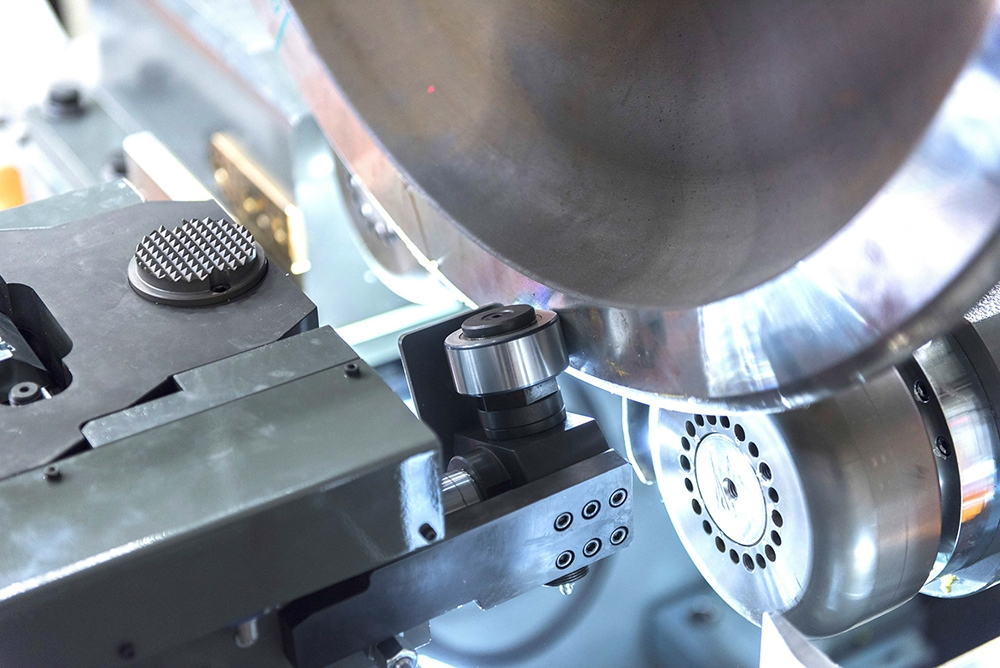
\includegraphics[width=.55\textwidth]{images/fig_00}
}%figues de la page de garde

\def\xxpied{%
Tour en fosse utilisé pour le reprofilage des roues ferroviaires\\
Concours Centrale Supelec -- PSI 2018%
}

\setcounter{secnumdepth}{5}
%---------------------------------------------------------------------------

\usepackage{bm}
\begin{document}
%\chapterimage{png/Fond_Cin}
\pagestyle{empty}


%%%%%%%% PAGE DE GARDE COURS
\ifcours
\begin{tikzpicture}[remember picture,overlay]
\node at (current page.north west)
{\begin{tikzpicture}[remember picture,overlay]
\node[anchor=north west,inner sep=0pt] at (0,0) {\includegraphics[width=\paperwidth]{\thechapterimage}};
\draw[anchor=west] (-2cm,-8cm) node [line width=2pt,rounded corners=15pt,draw=ocre,fill=white,fill opacity=0.6,inner sep=40pt]{\strut\makebox[22cm]{}};
\draw[anchor=west] (1cm,-8cm) node {\huge\sffamily\bfseries\color{black} %
\begin{minipage}{1cm}
\rotatebox{90}{\LARGE\sffamily\textsc{\color{ocre}\textbf{\xxnumpartie}}}
\end{minipage} \hfill
\begin{minipage}[c]{14cm}
\begin{titrepartie}
\begin{flushright}
\renewcommand{\baselinestretch}{1.1} 
\Large\sffamily\textsc{\textbf{\xxpartie}}
\renewcommand{\baselinestretch}{1} 
\end{flushright}
\end{titrepartie}
\end{minipage} \hfill
\begin{minipage}[c]{3.5cm}
{\large\sffamily\textsc{\textbf{\color{ocre} \discipline}}}
\end{minipage} 
 };
\end{tikzpicture}};
\end{tikzpicture}


\begin{tikzpicture}[overlay]
\node[shape=rectangle, 
      rounded corners = .25 cm,
	  draw= ocre,
	  line width=2pt, 
	  fill = ocre!10,
	  minimum width  = 2.5cm,
	  minimum height = 3cm,] at (18cm,0) {};
\node at (17.7cm,0) {\rotatebox{90}{\textbf{\Large\color{ocre}{\classe}}}};
%{};
\end{tikzpicture}

\vspace{3.5cm}

\begin{tikzpicture}[remember picture,overlay]
\draw[anchor=west] (-2cm,-6cm) node {\huge\sffamily\bfseries\color{black} %
\begin{minipage}{2cm}
\begin{center}
\LARGE\sffamily\textsc{\color{ocre}\textbf{\xxactivite}}
\end{center}
\end{minipage} \hfill
\begin{minipage}[c]{15cm}
\begin{titrechapitre}
\renewcommand{\baselinestretch}{1.1} 
\Large\sffamily\textsc{\textbf{\xxnumchapitre}}

\Large\sffamily\textsc{\textbf{\xxchapitre}}
\vspace{.5cm}

\renewcommand{\baselinestretch}{1} 
\normalsize\normalfont
\xxcompetences
\end{titrechapitre}
\end{minipage}  };
\end{tikzpicture}
\vfill

\begin{flushright}
\begin{minipage}[c]{.3\linewidth}
\begin{center}
\xxfigures
\end{center}
\end{minipage}\hfill
\begin{minipage}[c]{.6\linewidth}
\startcontents
\printcontents{}{1}{}
\end{minipage}
\end{flushright}

\begin{tikzpicture}[remember picture,overlay]
\draw[anchor=west] (4.5cm,-.7cm) node {
\begin{minipage}[c]{.2\linewidth}
\begin{flushright}

\includegraphics[width=2cm]{png/logoCC}
\end{flushright}
\end{minipage}
\begin{minipage}[c]{.2\linewidth}
\textsl{\xxauteur} \\
\textsl{\classe}
\end{minipage}
 };
\end{tikzpicture}
\newpage
\pagestyle{fancy}

\newpage
\pagestyle{fancy}

\else
\fi


%%%%%%%% PAGE DE GARDE TD
\iftd
%\begin{tikzpicture}[remember picture,overlay]
%\node at (current page.north west)
%{\begin{tikzpicture}[remember picture,overlay]
%\draw[anchor=west] (-2cm,-3.25cm) node [line width=2pt,rounded corners=15pt,draw=ocre,fill=white,fill opacity=0.6,inner sep=40pt]{\strut\makebox[22cm]{}};
%\draw[anchor=west] (1cm,-3.25cm) node {\huge\sffamily\bfseries\color{black} %
%\begin{minipage}{1cm}
%\rotatebox{90}{\LARGE\sffamily\textsc{\color{ocre}\textbf{\xxnumpartie}}}
%\end{minipage} \hfill
%\begin{minipage}[c]{13.5cm}
%\begin{titrepartie}
%\begin{flushright}
%\renewcommand{\baselinestretch}{1.1} 
%\Large\sffamily\textsc{\textbf{\xxpartie}}
%\renewcommand{\baselinestretch}{1} 
%\end{flushright}
%\end{titrepartie}
%\end{minipage} \hfill
%\begin{minipage}[c]{3.5cm}
%{\large\sffamily\textsc{\textbf{\color{ocre} \discipline}}}
%\end{minipage} 
% };
%\end{tikzpicture}};
%\end{tikzpicture}

%%%%%%%%%% PAGE DE GARDE TD %%%%%%%%%%%%%%%
%\begin{tikzpicture}[overlay]
%\node[shape=rectangle, 
%      rounded corners = .25 cm,
%	  draw= ocre,
%	  line width=2pt, 
%	  fill = ocre!10,
%	  minimum width  = 2.5cm,
%	  minimum height = 2.5cm,] at (18.5cm,0) {};
%\node at (17.7cm,0) {\rotatebox{90}{\textbf{\Large\color{ocre}{\classe}}}};
%%{};
%\end{tikzpicture}

% PARTIE ET CHAPITRE
%\begin{tikzpicture}[remember picture,overlay]
%\draw[anchor=west] (-1cm,-2.1cm) node {\large\sffamily\bfseries\color{black} %
%\begin{minipage}[c]{15cm}
%\begin{flushleft}
%\xxnumchapitre \\
%\xxchapitre
%\end{flushleft}
%\end{minipage}  };
%\end{tikzpicture}

% Bandeau titre exo
\begin{tikzpicture}[remember picture,overlay]
\draw[anchor=west] (-2cm,-6cm) node {\huge\sffamily\bfseries\color{black} %
\begin{minipage}{5cm}
\begin{center}
\LARGE\sffamily\color{ocre}\textbf{\textsc{\xxactivite}}

\begin{center}
\xxfigures
\end{center}

\end{center}
\end{minipage} \hfill
\begin{minipage}[c]{12cm}
\begin{titrechapitre}
\renewcommand{\baselinestretch}{1.1} 
\large\sffamily\textbf{\textsc{\xxtitreexo}}

\small\sffamily{\textbf{\textit{\color{black!70}\xxsourceexo}}}
\vspace{.5cm}

\renewcommand{\baselinestretch}{1} 
\normalsize\normalfont
\xxcompetences
\end{titrechapitre}
\end{minipage}  };
\end{tikzpicture}

\else
\fi


%%%%%%%% PAGE DE GARDE FICHE
\iffiche
\begin{tikzpicture}[remember picture,overlay]
\node at (current page.north west)
{\begin{tikzpicture}[remember picture,overlay]
\draw[anchor=west] (-2cm,-3.25cm) node [line width=2pt,rounded corners=15pt,draw=ocre,fill=white,fill opacity=0.6,inner sep=40pt]{\strut\makebox[22cm]{}};
\draw[anchor=west] (1cm,-3.25cm) node {\huge\sffamily\bfseries\color{black} %
\begin{minipage}{1cm}
\rotatebox{90}{\LARGE\sffamily\textsc{\color{ocre}\textbf{\xxnumpartie}}}
\end{minipage} \hfill
\begin{minipage}[c]{14cm}
\begin{titrepartie}
\begin{flushright}
\renewcommand{\baselinestretch}{1.1} 
\large\sffamily\textsc{\textbf{\xxpartie} \\} 

\vspace{.2cm}

\normalsize\sffamily\textsc{\textbf{\xxnumchapitre -- \xxchapitre}}
\renewcommand{\baselinestretch}{1} 
\end{flushright}
\end{titrepartie}
\end{minipage} \hfill
\begin{minipage}[c]{3.5cm}
{\large\sffamily\textsc{\textbf{\color{ocre} \discipline}}}
\end{minipage} 
 };
\end{tikzpicture}};
\end{tikzpicture}


\begin{tikzpicture}[overlay]
\node[shape=rectangle, 
      rounded corners = .25 cm,
	  draw= ocre,
	  line width=2pt, 
	  fill = ocre!10,
	  minimum width  = 2.5cm,
%	  minimum height = 2.5cm,] at (18.5cm,0.5cm) {};
	  minimum height = 2.5cm,] at (18.5cm,0cm) {};
\node at (17.7cm,0) {\rotatebox{90}{\textsf{\textbf{\large\color{ocre}{\classe}}}}};
%{};
\end{tikzpicture}



\else
\fi



\vspace{4.5cm}
\pagestyle{fancy}
\thispagestyle{plain}


\def\columnseprulecolor{\color{ocre}}
\setlength{\columnseprule}{0.4pt} 

\section{Contexte et étude préliminaire}

\begin{obj}
Valider la pertinence de l’utilisation d’une machine spéciale appelée tour en fosse pour le reprofilage
des roues ferroviaires.
\end{obj}

\subparagraph{}

\begin{itemize}
\item Pour la méthode $a$, $t_{i1} = t_3 +t_4 = \SI{14}{h}= \SI{840}{min}$.
\item Pour la méthode $b$, $t_{i2} = \left( 6\times 3 \times 2 \right)t_5 +t_6 = \SI{545}{min}$.
\end{itemize}

Le gain de temps $\Delta t_i = t_{i1}-t_{i2}=\SI{295}{min}$ soit \SI{4}{h} et \SI{55}{min}. C'est autant de temps gagner sur l'exploitation de la rame. 


.

\section{Analyse de l’entraînement en rotation d’une roue}
\subsection{Description fonctionnelle et structurelle du tour en fosse}
\subsection{Modélisation du dispositif de mise en rotation d’une roue}


\begin{obj}
Vérifier que la modélisation et les hypothèses retenues permettent de déterminer toutes les actions mécaniques nécessaires pour dimensionner les actionneurs des chaines d’énergie.
\end{obj}

\subparagraph{}
À partir des informations données, on peut réaliser le graphe de structure suivant. 

\begin{center}
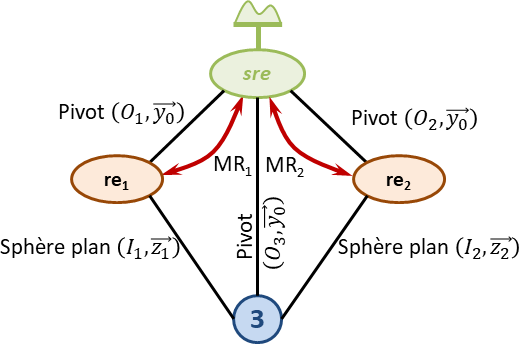
\includegraphics[width=.7\linewidth]{images/fig_02}
%\textit{}
\end{center}
\begin{multicols}{2}
\textbf{Méthode cinématique}
\begin{itemize}
\item Nombre cyclomatique $\gamma = L-S+1 $ avec $L=5$ liaisons et $S=4$ solides, on a donc $\gamma = 5-4+1=2$ et $E_c=12$ équations cinématiques.
\item Nombre d'inconnues cinématiques : 
\begin{itemize}
\item 3 liaisons pivot : $1\times 3=3$ inconnues;
\item 2 liaisons sphère-plan : $5\times 2=10$ inconnues;
\item \textbf{au total : $I_c=13$ inconnues cinématiques}.
\end{itemize}
\item Mobilités : 
\begin{itemize}
\item mobilités utiles : $m_u=2$ : entraînement des deux moteurs;
\item mobilités internes : en considérant le glissement entre la roue et les rouleaux, la roue 3, ainsi que $re_1$ et $re_2$ les rouleaux peuvent tourner librement. On a donc : $m_i =3$. %Dans le cas du roulement sans glissement, $m_i=3$;
\item au final, selon les hypothèses, $m=m_i+m_u=5$.
\end{itemize}
\item On a donc $h=m-I_c+E_c =5-13+12=4$.
\end{itemize}

\vfill\null
\columnbreak

\textbf{Méthode statique}
\begin{itemize}
\item 3 solides peuvent être isolés, $E_s=3\times 6 =18$ équations statiques.
\item Nombre d'inconnues statiques : 
\begin{itemize}
\item 3 liaisons pivot : $5\times 3=15$ inconnues;
\item 2 liaisons sphère-plan : $1\times 2=2$ inconnues;
\item \textbf{au total : $I_s=17$ inconnues statiques}.
\end{itemize}
\item Mobilités : $m=m_i+m_u=5$.
\item On a donc $h=m-E_S+I_s =5-18+17=4$.
\end{itemize}
\end{multicols}




%\textbf{Sans tenir compte que les solides 1, 2 et sre sont encastrés au bâti, on est dans les conditions suivantes.}
%
%\begin{center}
%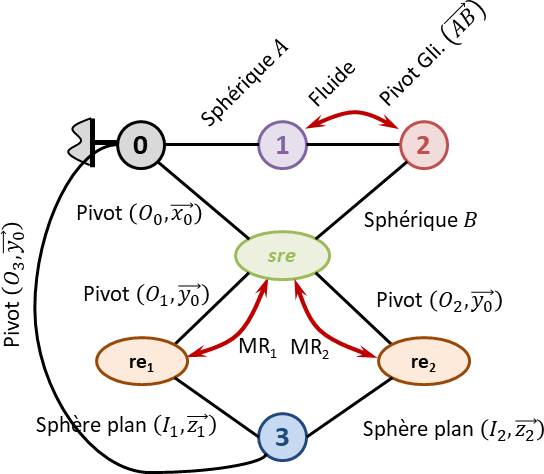
\includegraphics[width=.7\linewidth]{images/fig_01}
%%\textit{}
%\end{center}
%\begin{multicols}{2}
%\textbf{Méthode cinématique}
%\begin{itemize}
%\item Nombre cyclomatique $\gamma = L-S+1 $ avec $L=9$ liaisons et $S=7$ solides, on a donc $\gamma = 9-7+1=3$ et $E_c=18$ équations cinématiques.
%\item Nombre d'inconnues cinématiques : 
%\begin{itemize}
%\item 2 liaisons sphériques : $3\times 2=6$ inconnues;
%\item 4 liaisons pivot : $1\times 4=4$ inconnues;
%\item 1 liaison pivot glissant : 2 inconnues;
%\item 2 liaisons sphère-plan : $5\times 2=10$ inconnues;
%\item \textbf{au total : $I_c=22$ inconnues cinématiques}.
%\end{itemize}
%\item Mobilités : 
%\begin{itemize}
%\item mobilités utiles : $m_u=3$ : entrainement des deux moteurs ainsi que le déploiement du vérin;
%\item mobiltés internes : en considérant le glissement entre la roue et les rouleaux, la roue 3, ainsi que $re_1$ et $re_2$ les rouleaux peuvent tourner librement, rotation propre de la pièce 1 et de la pièce 2 autour du vecteur $\vect{AB}$. On a donc : $m_i =5$. %Dans le cas du roulement sans glissement, $m_i=3$;
%\item au final, selon les hypothèses, $m=m_i+m_u=8$.
%\end{itemize}
%\item On a donc $h=m-I_c+E_c =8-22+18=4$.
%\end{itemize}
%
%\vfill\null
%\columnbreak
%
%\textbf{Méthode statique}
%\begin{itemize}
%\item 6 solides peuvent être isolés, $E_s=6\times 6 =36$ équations statiques.
%\item Nombre d'inconnues statiques : 
%\begin{itemize}
%\item 2 liaisons sphériques : $3\times 2=6$ inconnues;
%\item 4 liaisons pivot : $5\times 4=20$ inconnues;
%\item 1 liaison pivot glissant : 4 inconnues;
%\item 2 liaisons sphère-plan : $1\times 2=2$ inconnues;
%\item \textbf{au total : $I_s=32$ inconnues statiques}.
%\end{itemize}
%\item Mobilités : $m=m_i+m_u=9$.
%\item On a donc $h=m-E_S+I_s =8-36+32=4$.
%\end{itemize}
%\end{multicols}
%
%En utilisant la condition de roulement sans glissement et la méthode cinématique, on ajoute 2 équations cinématiques et $h=3$.

\subparagraph{}
%\begin{multicols}{2}
Condition de roulement sans glissement en $I_1$ : $\vectv{I_1}{3}{re_1} = \vect{0} \Leftrightarrow \vectv{I_1}{3}{0}-\vectv{I_1}{re_1}{0} = \vect{0}$. Par suite, 
\begin{itemize}
\item $\vectv{I_1}{3}{0}=\vectv{O_3}{3}{0}+\vect{I_1 O_3}\wedge \vecto{3}{0} = R\vect{z_1} \wedge \omega_3\vect{y_0}=-R\omega_3 \vect{x_1}$;
\item $\vectv{I_1}{re_1}{0}=\vectv{O_1}{3}{0}+\vect{I_1 O_1}\wedge \vecto{3}{0} = -R_{re}\vect{z_1} \wedge \omega_{re_1}\vect{y_0}=R_{re}\omega_{re_1} \vect{x_1}$.
\end{itemize}
On a donc $-R\omega_3 -R_{re}\omega_{re_1} =0 \Leftrightarrow\dfrac{\omega_3}{\omega_{re_1}}=-\dfrac{R_{re}}{R} $.
%\end{multicols}

De même en exploitant le roulement sans glissement en $I_2$, $\dfrac{\omega_3}{\omega_{re_2}}=-\dfrac{R_{re}}{R} $. 

La condition de roulement sans glissement supprime les 3 mobilités internes; donc $m'=2$ et $h'=1$. 

\subparagraph{}
Dans les conditions précédentes, les couples $\mathcal{C}_{mi}$ ne peuvent pas être déterminés. Il faudrait imposer un taux de rotation rigoureusement identique pour $\omega_{re_1}$ et $\omega_{re_2}$. 


\subsection{Motorisation du dispositif de mise en rotation d'une roue}
\begin{obj}
Analyser la chaîne d’entraînement en rotation d’une roue et vérifier le choix de la machine électrique.
\end{obj}

\subparagraph{}
On conserve l'hypothèse que $sre$ est supposé fixe par rapport au bâti. 
On a $E_1=M_1+R_1+re_1$. Ces 3 solides sont en liaison pivot par rapport au bâti. En conséquence, 
$T\left(E_1/0\right)=T\left(M_1/0\right)+T\left(R_1/0\right)+T\left(re_1/0\right) = \dfrac{1}{2}J_m\omega_m^2+\dfrac{1}{2}J_{re}\omega_{re}^2+\dfrac{1}{2}J_{re}\omega_{re}^2=\dfrac{1}{2}\left(J_m+J_{red}k^2+J_{re}k^2\left( \dfrac{R_{re}}{R}\right)^2 \right) \omega_m^2$.

On a donc $J_{eq}=J_m+J_{red}k^2+J_{re}k^2\left( \dfrac{R_{re}}{R}\right)^2$.

\subparagraph{}
On prend le graphe de structure suivant :
\begin{center}
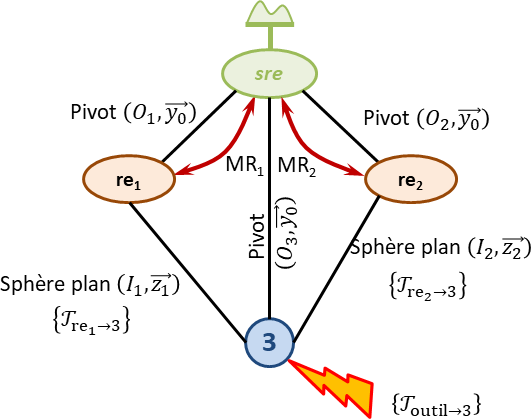
\includegraphics[width=.5\linewidth]{images/fig_03}
%\textit{}
\end{center}

On isole $E_1$. Bilan des puissances internes : les liaisons internes au système considrée sont considérées sans frottement. On a donc : $\mathcal{P}_{\text{int}}\left(E_1\right)=0$.

Bilan des puissances externes : 
\begin{itemize}
\item la puissance développée par le moteur peut s'exprimer par $\mathcal{P}\left(\text{sre}\to M_1/0\right)=C_m\omega_m$;
\item puissance développée par l'action de 3 sur $\text{re}_1$ : $\mathcal{P}\left(3\to \text{re}_1/0\right)=\torseurcin{V}{\text{re}_1}{0}\otimes\torseurstat{T}{3}{\text{re}_1}=\torseurl{k\omega_m \vect{y_0}}{kR_{re}\omega_m\vect{x_1}}{I_1}\otimes
\torseurl{-F_{z1}\vect{z_1}-F_{x1}\vect{x_1}}{\vect{0}}{I_1}= -kR_{re}F_{x1}\omega_m$.
\end{itemize}

On applique le théorème de l'énergie cinétique et $\dfrac{\dd T\left(E_1/0\right)}{\dd t}= C_m\omega_m-kR_{re}F_{x1}\omega_m \Rightarrow \dot{\omega}_m J_{eq}= C_m-kR_{re}F_{x1} $.

\subparagraph{}
En isolant l'ensemble $E_2=\left\{M_2+R_2+re_2\right\}$ et en appliquant le théorème de l'énergie cinétique : $\dot{\omega}_m J_{eq}= C_m-kR_{re}F_{x2}$. Comme les caractéristiques des deux chaînes d’entraînement sont les mêmes, on a donc nécessairement $F_{x1}=F_{x2}$.

\subparagraph{}
On a vu que $\dfrac{\omega_3}{\omega_{re_1}}=-\dfrac{R_{re}}{R}$ de plus $\omega_{re_1}=k\omega_m$; donc $\omega_3= -k\dfrac{R_{re}}{R}\omega_m$. En dérivant, on a $\dot{\omega_3}= -k\dfrac{R_{re}}{R}\dot{\omega}_m$.


\subparagraph{}
\textbf{Stratégie :} on cherche à exprimer le couple moteur en fonction des grandeurs du géométriques, inertielles, ... pour cela, la roue étant en pivot d'axe $\axe{O}{y_0}$ on va réaliser un théorème du moment dynamique en $O_3$ en projection sur $\vect{y_0}$. 

On isole la roue \textbf{3}.

On réalise le bilan des actions mécaniques extérieures : 
\begin{itemize}
\item action de la pivot en $O_3$ (pas de moment en $O_3$ en projection sur $\vect{y_0}$);
\item action des liaisons sphères plans : 
\begin{itemize}
\item $\vectm{O_3}{re_1}{3}\cdot \vect{y_0} = \left(\vect{O_3 I_1} \wedge \left(  F_{x1}\vect{x_1}+F_{z1}\vect{z_1}\right) \right) \cdot \vect{y_0}
= \left(-R\vect{z_1} \wedge \left(  F_{x1}\vect{x_1}+F_{z1}\vect{z_1}\right) \right) \cdot \vect{y_0}
= -RF_{x1}$.
\item $\vectm{O_3}{re_2}{3}\cdot \vect{y_0} 
= \left(\vect{O_3 I_2} \wedge \left(  F_{x2}\vect{x_2}+F_{z2}\vect{z_2}\right) \right) \cdot \vect{y_0}
= \left(-R\vect{z_2} \wedge \left(  F_{x2}\vect{x_2}+F_{z2}\vect{z_2}\right) \right) \cdot \vect{y_0}
= -RF_{x2}$.
\end{itemize}
\item action de l'outil :
$\vectm{O_3}{\text{outil}}{3}\cdot \vect{y_0} 
= \left(\vect{O_3 C} \wedge \vectf{\text{outil}}{3} \right) \cdot \vect{y_0}
= \left(\left( -\lambda(t) \vect{y_0}-R_C(t) \vect{z_0}\right) \wedge \vectf{\text{outil}}{3} \right) \cdot \vect{y_0}
= \left( -\lambda(t) \vect{y_0}\wedge \vectf{\text{outil}}{3}-R_C(t) \vect{z_0} \wedge \vectf{\text{outil}}{3}\right)   \cdot \vect{y_0}
= \left(-R_C(t) \vect{z_0} \wedge \vectf{\text{outil}}{3} \right) \cdot \vect{y_0}
= -R_C(t)\left( \vect{y_0} \wedge \vect{z_0} \right) \cdot \vectf{\text{outil}}{3}
= -R_C(t) \vect{x_0}  \cdot \vectf{\text{outil}}{3}=R_C(t) f_{ex}
%= \left( \vectf{\text{outil}}{3} \wedge \vect{y_0}\right) \cdot \vect{O_3 C}
%= \left( \vectf{\text{outil}}{3} \wedge \vect{y_0}\right) \cdot \vect{O_3 C}
$.
\end{itemize}

Enfin, la roue étant supposée équilibrée, on a $\vectmd{O_3}{3}{0}\cdot\vect{y_0}=J_3\ddot{\omega}_3$.


Le TMD appliqué en 3 en projection sur $\vect{y_0}$  est donné par 
$J_3\ddot{\omega}_3=-2RF_{x1}+R_C(t) f_{ex}$. De plus, 
$\omega_3= -k\dfrac{R_{re}}{R}\omega_m$ et 
$\dot{\omega}_m J_{eq}= C_m-kR_{re}F_{x1} \Leftrightarrow F_{x1}= \dfrac{C_m-\dot{\omega}_m J_{eq}}{kR_{re}}$.

Au final :
$$-J_3k\dfrac{R_{re}}{R}\dot{\omega}_m=-2R\dfrac{C_m-\dot{\omega}_m J_{eq}}{kR_{re}}+R_C(t) f_{ex} \Leftrightarrow
C_m=\dot{\omega}_m J_{eq}
+J_3k^2\dfrac{R_{re}^2}{2R^2}\dot{\omega}_m+ \dfrac{R_C(t) kR_{re} f_{ex}}{2R}.$$

%En faisant l'hypothèse que le moteur tourne dans le sens direct, la roue tourne dans le sens horaire. On peut alors déduire les signes des efforts normaux et tangentiels. Ainis, $F_{x1}=-f F_{z1}$. 
%
%
%\begin{center}
%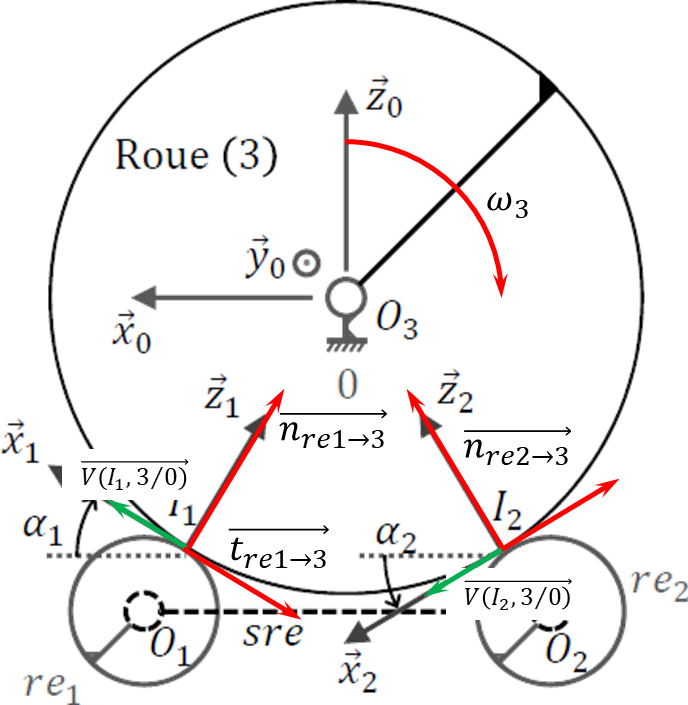
\includegraphics[width=.5\linewidth]{images/fig_04}
%%\textit{}
%\end{center}
%
% 
%Ainsi :
%\begin{itemize}
%\item $\torseurstat{T}{re_1}{3} = \torseurl{F_{z1}\vect{z_1}+F_{x1}\vect{x_1}}{\vect{0}}{I_1}$. 
%\end{itemize}

\subparagraph{}
En utilisant l'expression précédente, le couple est maximum lorsque $R_C(t)=R_M$.

\subparagraph{}
En utilisant la décomposition du vecteur vitesse, 
$\vectv{C}{\text{outil}}{3}=\vectv{C}{\text{outil}}{0}-\vectv{C}{\text{3}}{0}$. 
D'après le document réponse, $\vectv{C}{\text{outil}}{0}=V_f(t)\vect{u}=-b\omega_3\vect{u}$. Par ailleurs, $\vectv{C}{\text{3}}{0}=R_C(t)\omega_3\vect{x_0}$.

Au final, $\vectv{C}{\text{outil}}{3}=V_f(t)\vect{u}-R_C(t)\omega_3\vect{x_0}$.

$\vectv{C}{\text{outil}}{3} \cdot \vect{x_0} = -V_C =  V_f(t)\vec t{u}\cdot \vect{x_0}-R_C(t)\omega_3 = -R_C(t)\omega_3$. On a donc $V_C=R_C(t)\omega_3$. Ainsi : 
\begin{itemize}
\item $V_C=R_C(t)\omega_3(t)=R_M \omega_{C_0}\Rightarrow \omega_{C_0}=\dfrac{V_C}{R_M}$.
\item $V_C=R_C(t)\omega_3(t)=R_m \omega_{C_1}\Rightarrow \omega_{C_1}=\dfrac{V_C}{R_m}$.
\end{itemize}
 
 \subparagraph{}
 
 \begin{center}
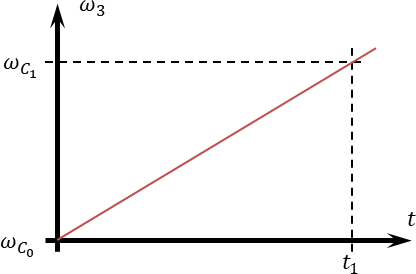
\includegraphics[width=.5\linewidth]{images/fig_05}
%\textit{}
\end{center}

Dans ces conditions, on a $\omega_3(t)=\dfrac{\omega_{C_1}-\omega_{C_0}}{t_1}t+\omega_{C_0}$.

\subparagraph{} %Q13
On a $l(t)=||\vect{C_0C}||=||\int\limits_0^t V_f(t)\vect{u} \dd t||=||\int\limits_0^t -b\omega_3(t) \vect{u} \dd t||$ 
$=||\int\limits_0^t -b\left( \dfrac{\omega_{C_1}-\omega_{C_0}}{t_1}t+\omega_{C_0}\right) \vect{u} \dd t||$

$=b|| \left(  \dfrac{\omega_{C_1}-\omega_{C_0}}{2t_1}t^2+\omega_{C_0}t\right) \vect{u} ||$.

Au final, 
$l(t)=b \left(  \dfrac{\omega_{C_1}-\omega_{C_0}}{2t_1}t^2+\omega_{C_0}t\right) $.


\subparagraph{} %Q14
D'après la figure, on a  $l(t_1)=||\vect{C_0C_1}||=\sqrt{\left(R_M-R_m \right)^2+e^2}$.

On a donc $l(t_1)=b \left(  \dfrac{\omega_{C_1}-\omega_{C_0}}{2t_1}t_1^2+\omega_{C_0}t_1\right) =\sqrt{\left(R_M-R_m \right)^2+e^2}$ 
$\Leftrightarrow 
  t_1 \left(\dfrac{\omega_{C_1}-\omega_{C_0}}{2}+\omega_{C_0}\right) =\dfrac{\sqrt{\left(R_M-R_m \right)^2+e^2}}{b}$.

$\Leftrightarrow 
  t_1  =\dfrac{\sqrt{\left(R_M-R_m \right)^2+e^2}}{b} \dfrac{2}{\omega_{C_1}+\omega_{C_0}}$.


\subparagraph{} %Q15

En dérivant l'expression obtenue à la question 12, on a 
$\dot{\omega}_3(t)=\dfrac{\omega_{C_1}-\omega_{C_0}}{t_1} =  \dfrac{b\left( \omega_{C_1}+\omega_{C_0}\right)\left( \omega_{C_1}-\omega_{C_0}\right)}{2\sqrt{\left(R_M-R_m \right)^2+e^2}}  $. 

Au final, $\dot{\omega}_3(t) =\dfrac{b\left( \omega_{C_1}^2-\omega_{C_0}^2\right)}{2\sqrt{\left(R_M-R_m \right)^2+e^2}}  $. 

\subparagraph{} %Q16

D'après les annexes, on a $R_m=\SI{0,4}{m}$ et $V_C=\SI{400}{m.min^{-1}}$. On a donc $N_3=\dfrac{V_c}{\pi \cdot 2 R_m} = \dfrac{400}{0,8\pi} = \SI{159}{tr.min^{-1}}$. On a donc $N_m = N_3 \dfrac{R}{kR_e}=159 \dfrac{0,47}{0,1\cdot 0,175} = \SI{4275}{tr.min^{-1}}$. Le moteur doit donc pouvoir tourner au moins à cette vitesse.

On ne sait pas si le couple moteur maximum calculé (\SI{22}{Nm}) tient compte du rendement. 
S'il tient compte du rendement, le moteur ME\_10\_10 convient. Sinon, il faudra utiliser le ME\_5\_15. 

\section{Analyse de la commande du dispositif de mise en translation de l’outil}
\begin{obj}
Analyser la chaîne d’asservissement en position et en vitesse du porte-outil afin de proposer puis de régler un correcteur permettant d’assurer le niveau de précision attendu pour le profil de la roue.
\end{obj}

\subsection{Effet de la déformation de l’outil sur la forme de la roue reprofilée}

\subparagraph{} %Q17. 

Graphiquement on a :
\begin{itemize}
\item $\Delta u_1 = \Delta z_2 \simeq \SI{5}{\mu m}$;
\item $R^2 + \Delta x_2^2 = \left(R + \Delta u_2\right)^2$ soit $\Delta u_2 = \sqrt{R^2 + \Delta x_2^2} - R = \sqrt{0,47^2 + 0,0005^2} - 0,47 \simeq \SI{0,27}{\mu m}$.%\simeq R\left(1+\dfrac{\Delta x_2^2}{2R^2}\right) - R \simeq \dfrac{\Delta x_2^2}{2R}$.
\end{itemize}
Il y a un rapport de 18,8 entre le défaut dû à la compression et celui dû à la flexion. On néglige donc ce dernier. 
 

\subsection{Analyse d’une solution avec un porte-outil fixé au bâti}
\begin{obj}
Déterminer les variations de position du point de contact $C$ entre la roue et l’outil pour une variation
sinusoïdale de l’effort perturbateur $f_c(t)$.
\end{obj}


\subparagraph{VALEURS A REVOIR} %Q18
~\\

On isole l'outil. Celui-ci est soumis :
\begin{itemize}
\item à l'action du ressort suivant $\vect{z_0}$ : $-Kz_2(t)$;
\item à l'action de l'amortisseur $\vect{z_0}$ : $-\lambda \dot{z}_2(t)$;
\item à l'action de l'effort perturbateur $\vect{z_0}$ : $f_c(t)$. 
\end{itemize}

En appliquant le théorème de la résultante dynamique suivant $\vect{z_0}$ on obtient : $-Kz_2(t)-\lambda \dot{z}_2(t)+f_c(t)=m_2\ddot{z}_2(t)$.

En utilisant la transformée de Laplace, on obtient alors 
$-KZ_2(p)-\lambda p{Z}_2(p)+F_c(p)=m_2p^2{Z}_2(p) \Leftrightarrow S(p)=\dfrac{Z_2(p)}{F_c(p)}=\dfrac{1}{K+\lambda p  + m_2 p^2}
$.

En mettant cette fonction de transfert sous forme canonique, on a 
$K_S =1/K \simeq \SI{3,57e-8}{m.N^{-1}}$, 
$\omega_{0S}^2 = \dfrac{K}{m_2} \Rightarrow \omega_{0S}\simeq \SI{188,5}{rad.s^{-1}}$ et 
$\dfrac{2\xi_S}{\omega_{0S}} = \dfrac{\lambda}{K} \Leftrightarrow \xi_S = \dfrac{\lambda }{2\sqrt{Km_2}} \simeq 0,1$.

L'amplitude maximale est donnée par : $A_{\text{max}}=\dfrac{K_S}{2\xi_S\sqrt{1-\xi_S^2}}\simeq \dfrac{3,57\cdot 10^{-8}}{0,2\sqrt{1-0,01}}=1,8\cdot 10^{-7}$.


%%<<<<<<< HEAD
%%=======

La pulsation de résonance est donnée par $\omega_r = \omega_{0S} \sqrt{1-2\xi^2} = 188,5\sqrt{1-2\times 0,1^2}=\SI{186,6}{rad.s^{-1}}$.



Pour une entrée valant $f_c(t)=\left(f_{c0}+f_{c1}\sin \left(\omega t\right)\right) \mathcal{H}(t)$, en utilisant le théorème de superposition, on obtient en régime permanent le signal suivant : 
$z_2(t)=K_S f_{c0}  + f_{c1} A_{\text{max}} \sin \left(\omega_r t+\varphi\right)$ avec $\varphi=90\degres$.

Dans ces conditions on a donc $\Delta z_2 = 2 f_{c1} A_{\text{max}}\simeq \SI{3.6000e-05}{m} \simeq {36}{\mu m} $. Le cahier des charges n'est donc pas respecté ($\Delta u$ doit être inférieur à $\SI{30}{\mu m}$).
\begin{center}
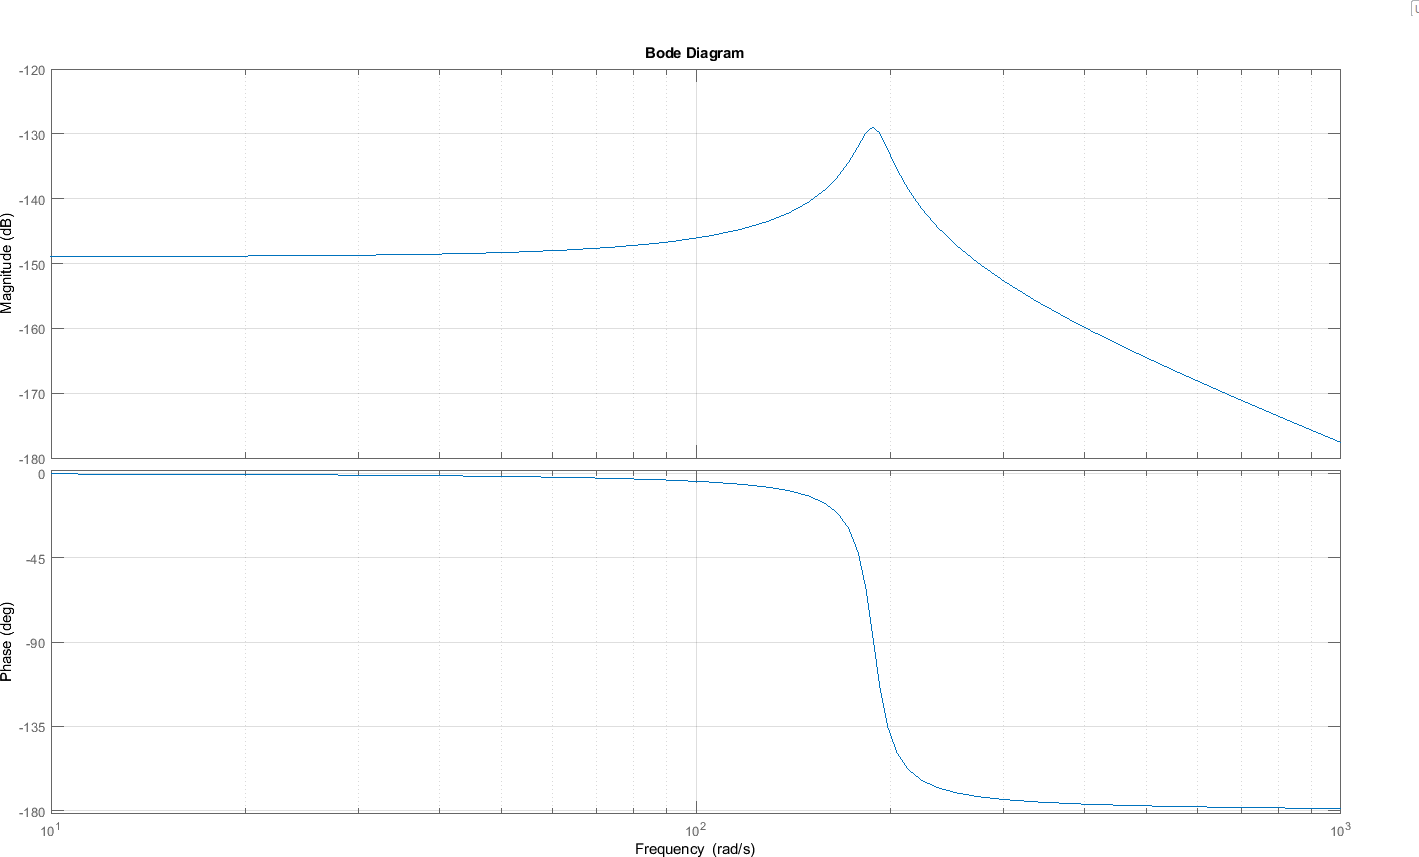
\includegraphics[width=.8\linewidth]{images/fig_08}
\end{center}

%%>>>>>>> a67712ce21440b340ba6bc731e97b873a885f38e

\subsection{Analyse des asservissements du porte-outil}
\subsubsection{Modélisation du mouvement pour la commande}

\begin{obj}
Modéliser le comportement dynamique de l’outil et du porte-outil, puis étudier une commande  en position $z_1(t)$ comprenant un correcteur proportionnel.
\end{obj}

\subparagraph{}

D'après le schéma-blocs $Z_1(p)=H_2(p)\left(F_m(p)+H_1(p)Z_2(p)\right)$. 
D'après la première équation différentielle, on a : $m_1p^2 Z_1(p) + \lambda pZ_1(p)+KZ_1(p)=\lambda pZ_2(p)+KZ_2(p)+F_m(p)\Leftrightarrow 
Z_1(p)\left(m_1p^2  + \lambda p+K \right)=Z_2(p)\left(\lambda p+K\right)+F_m(p)
\Leftrightarrow 
Z_1(p)= \dfrac{Z_2(p)\left(\lambda p+K\right)+F_m(p)}{m_1p^2  + \lambda p+K}$.
On a donc par identification $H_2(p)=\dfrac{1}{m_1p^2  + \lambda p+K}$ et $H_1(p)=\lambda p+K$.

D'après le schéma-blocs $Z_2(p)=H_4(p)\left(F_c(p)+H_3(p)Z_1(p)\right)$. D'après la seconde équation différentielle,  $m_2p^2 Z_2(p) + \lambda pZ_2(p)+KZ_2(p)=\lambda pZ_1(p)+KZ_1(p)+F_C(p)\Leftrightarrow Z_2(p)\left( m_2p^2  + \lambda p+K \right)=Z_1(p)\left(\lambda p+K\right)+F_C(p)\Leftrightarrow Z_2(p)=\dfrac{Z_1(p)\left(\lambda p+K\right)+F_C(p)}{ m_2p^2  + \lambda p+K}$.
On a donc par identification $H_4(p)=\dfrac{1}{m_2p^2  + \lambda p+K}$ et $H_3(p)=\lambda p+K$.



\subparagraph{}
En utilisant le premier modèle, on avait :
$
\left\{\begin{array}{l}
Z_1(p)=H_2(p)\left(F_m(p)+H_1(p)Z_2(p)\right) \\
Z_2(p)=H_4(p)\left(F_c(p)+H_3(p)Z_1(p)\right)
\end{array}
\right.
$. 

Ainsi, $Z_1(p)=H_2(p)\left(F_m(p)+H_1(p)\left( H_4(p)\left(F_c(p)+H_3(p)Z_1(p)\right)\right)\right) $

$=H_2(p)F_m(p)+H_1(p)H_2(p) H_4(p)F_c(p)+H_1(p)H_2(p) H_3(p)H_4(p)Z_1(p) $

$\Leftrightarrow Z_1(p)\left( 1-H_1(p)H_2(p) H_3(p)H_4(p)\right)=H_2(p)\left(F_m(p)+H_1(p)H_4(p)F_c(p)\right) $. 

En utilisant le schéma-blocs, $Z_1(p)=\left(F_c(p)N_1(p)+F_m(p)\right)N_2(p)$. 
Par identification, on obtient $N_1(p)=H_1(p)H_4(p)$ et $N_2(p)=\dfrac{H_2(p)}{1-H_1(p)H_2(p) H_3(p)H_4(p)}$.


\subparagraph{}

$N_2(p)=\dfrac{H_2(p)}{1-H_1(p)H_2(p) H_3(p)H_4(p)}$ 
$= \dfrac{\dfrac{1}{m_1p^2  + \lambda p+K}}{1-\left(\lambda p+K\right)\dfrac{1}{m_1p^2  + \lambda p+K} \left(\lambda p+K\right)\dfrac{1}{m_2p^2  + \lambda p+K}}$
$= \dfrac{1}{\left(m_1p^2  + \lambda p+K\right)- \dfrac{\left(\lambda p+K\right)^2}{m_2p^2  + \lambda p+K}}$

$= \dfrac{m_2p^2  + \lambda p+K}{\left(m_1p^2  + \lambda p+K\right)\left(m_2p^2  + \lambda p+K\right)- \left(\lambda p+K\right)^2}$
$= \dfrac{m_2p^2  + \lambda p+K}{
m_2m_1p^4  + \lambda m_1p^3+Km_1p^2+\lambda m_2p^3  + \lambda^2 p^2 +\lambda pK+Km_2p^2  + K\lambda p+K^2 - \lambda^2 p^2 -K^2 - 2\lambda p K}$

$= \dfrac{m_2p^2  + \lambda p+K}{
m_2m_1p^4  + \lambda m_1p^3+Km_1p^2+\lambda m_2p^3   +Km_2p^2 }$
$= \dfrac{m_2p^2  + \lambda p+K}{
p^2\left( m_1m_2p^2  + \left(m_1+ m_2\right) \lambda p  +K\left(m_1+m_2\right)\right) }$

$= \dfrac{m_2\left(p^2  + \dfrac{\lambda}{m_2}p+\dfrac{K}{m_2}\right)}{
p^2 m_1m_2 \left(p^2  + \dfrac{m_1+ m_2}{m_1m_2} \lambda p  +K\dfrac{m_1+m_2}{m_1m_2}\right) }$.

Par identification, on a : $A=\dfrac{1}{m_1}$, $\omega_1^2=\dfrac{K}{m_2}$, $2\xi_1\omega_1=\dfrac{\lambda}{m_2}$, $\omega_2^2=K\dfrac{m_1+m_2}{m_1m_2}$, $2\xi_2\omega_2=\lambda\dfrac{m_1+ m_2}{m_1m_2}$. 

On a donc $\xi_1=\dfrac{\lambda}{2  \sqrt{m_2K}}$ et 
$\xi_2=\lambda\dfrac{\sqrt{m_1+ m_2}}{2\sqrt{Km_1m_2}}$.



\subparagraph{}
D'après le diagramme asymptotique donné, on a nécessairement $\omega_1<\omega_2$. On peut dresser un tableau des variations à partir de la fonction de transfert $N_2(p)$. 
\begin{center}
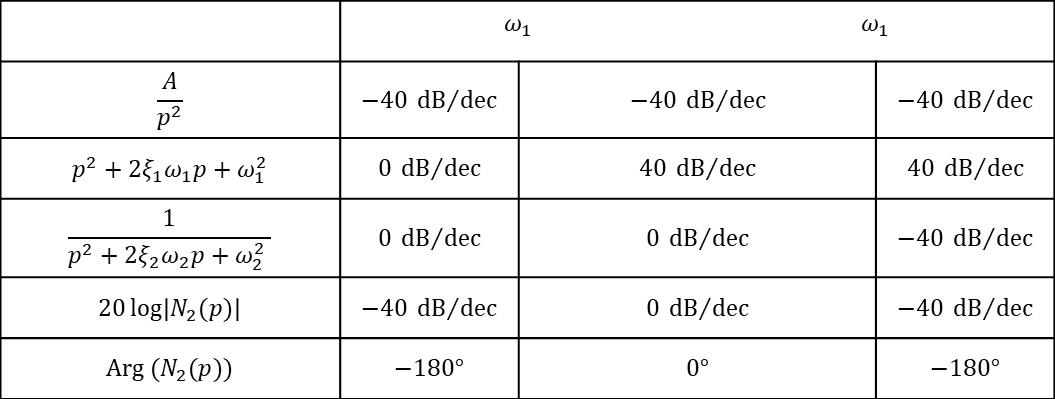
\includegraphics[width=.7\linewidth]{images/fig_06}

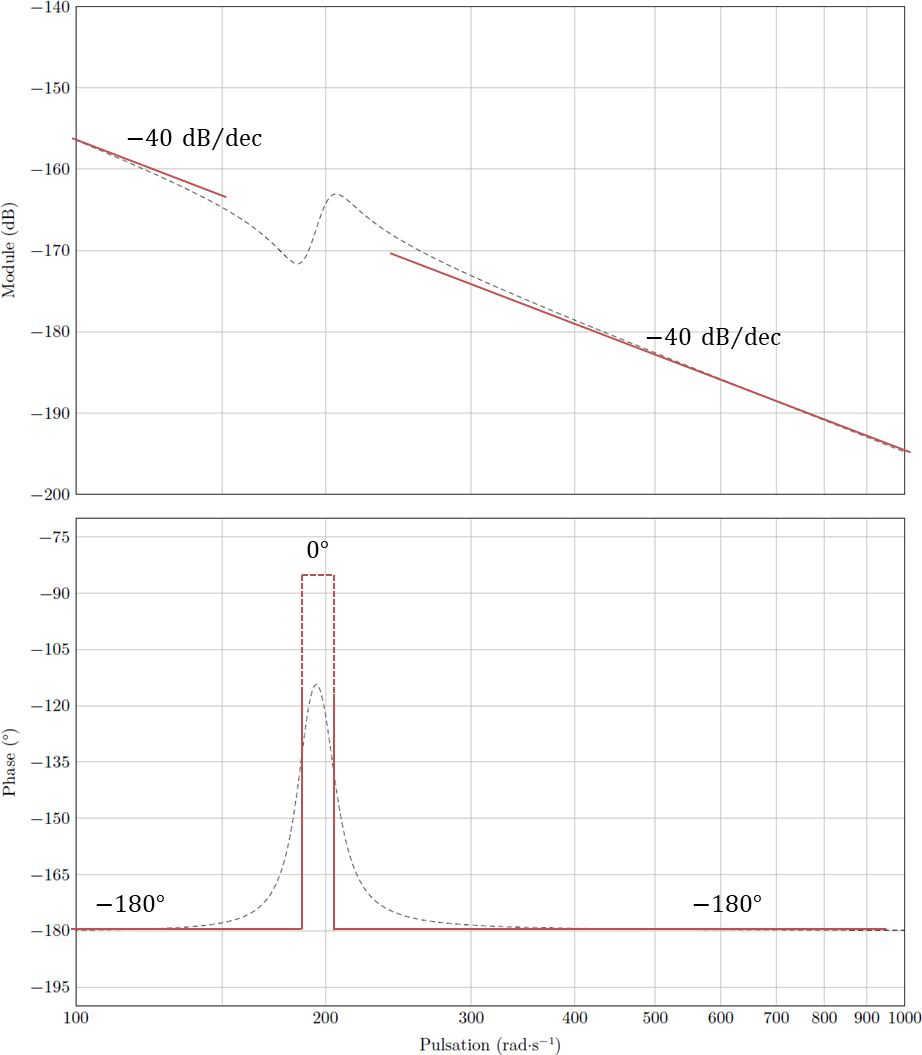
\includegraphics[width=.7\linewidth]{images/fig_07}
%\textit{}
\end{center}

\subparagraph{}
Si le système n'est pas sollicité par des pulsations comprises entre 150 et \SI{250}{rad.s^{-1}}, on peut modéliser $N_2(p)$ par un double intégrateur. 
Le gain dB est donc  $20\log A - 20 \log \omega^2$.  Pour $\omega=\SI{500}{rad.s^{-1}}$ on a $20\log A - 20 \log 500^2=-182,5 \Rightarrow \log A = \dfrac{20 \log 500^2-182,5}{20}$ et $A=1,87\cdot 10^{-4}$.


\subparagraph{}

%\subparagraph{}
Dans le cas, la FTBO est de classe 2.
\begin{itemize}
\item \textbf{req 1.1} : $M\varphi = 60\degres$ : impossible à respecter la phase sera toujours de $\SI{-180}{\degres}$.
\item \textbf{req 1.2} : $\omega_{\SI{0}{dB}}=\SI{200}{rad.s^{-1}}$ : critère non respecté (cf diagramme de Bode).
\item \textbf{req 1.4} : erreur en régime permanent : $\Delta c < \SI{40}{\mu m}$ pour un échelon d'amplitude $f_{c0}=\SI{1}{kN}$ : critère non respecté (pas d'intégrateur avant la perturbation).
\item \textbf{req 1.5} : défaut de la roue $\Delta u < \SI{30}{\mu m}$ lorsque la perturbation est sinusoïdale.
\end{itemize}

La correctioin proportionnelle ne permet donc pas de respecter tous les critères du cahier des charges.

\subsubsection{Calcul des paramètres des correcteurs de la loi de commande}

\begin{obj}
Déterminer les paramètres d’une loi de commande afin de valider les performances statiques et dynamiques du cahier des charges.
\end{obj}

\subparagraph{} %
On a $\arg \left(H_{\text{BO}}(j\omega)\right)=\arg\left(AK_v \right) + \arg\left(p+\dfrac{1}{T_i}\right) + \arg\left(p+K_p\right)-3 \arg(p)$
$ =\arctan T_i\omega +\arctan\omega/K_P -270$.

On souhaite que la marge de phase soit de 60\degres soit 
$\arg \left(H_{\text{BO}}(j\omega_{\SI{0}{dB}})\right)=-120\degres$. 
On a donc 
$-120=\arctan T_i\omega_{\SI{0}{dB}} +\arctan\omega_{\SI{0}{dB}}/K_P -270 \Leftrightarrow \arctan T_i\omega_{\SI{0}{dB}} +\arctan\omega_{\SI{0}{dB}}/K_P = 150$.

Or $\tan(a+b)=\dfrac{\tan a + \tan b}{1-\tan a\tan b}$. 

On a donc $\tan 150 = \dfrac{T_i\omega_{\SI{0}{dB}} + \omega_{\SI{0}{dB}}/K_P}{1-T_i\omega_{\SI{0}{dB}}^2/K_P}$
$ \Leftrightarrow \tan 150 -\tan 150 T_i\omega_{\SI{0}{dB}}^2/K_P= T_i\omega_{\SI{0}{dB}} + \omega_{\SI{0}{dB}}/K_P $

$ \Leftrightarrow  T_i  = \dfrac{K_P\tan 150 - \omega_{\SI{0}{dB}}}{K_P\omega_{\SI{0}{dB}}+\tan 150 \omega_{\SI{0}{dB}}^2}$.


\begin{rem} D'une part, en utilisant le schéma-blocs, on a :

$H_{\text{BO}}(p)=\dfrac{K_P}{p}\dfrac{H_{\text{PI}(p)}pN_{\text{2app}}(p)}{1+H_{\text{PI}(p)}pN_{\text{2app}}(p)}$
$=\dfrac{K_P}{p}\dfrac{K_v\left(1+\dfrac{1}{Ti_ p} \right)p\dfrac{A}{p^2}}{1+K_v\left(1+\dfrac{1}{Ti_ p} \right)p\dfrac{A}{p^2}}$
$=\dfrac{K_P}{p}\dfrac{K_v\left(T_i p+1 \right){A}}{T_i p^2+K_v\left(T_i p+1 \right){A}}$.
$=\dfrac{K_P}{p}\dfrac{T_i p+1}{\dfrac{T_i}{AK_v} p^2+ T_i p+1 }$.

D'autre part, en prenant la FTBO proposée, on a : 

$H_{\text{BO}}(p)=\dfrac{AK_v\left(p+\dfrac{1}{T_i} \right)\left(p+K_p\right)}{p^3}$
$=\dfrac{AK_v}{T_i}\dfrac{T_ip^2+T_iK_pp+p+K_p }{p^3}$
$=\dfrac{AK_v}{T_iK_p}\dfrac{\dfrac{T_i}{K_p}p^2+T_ip+p+1 }{p^3}$.

La forme proposée par le sujet et la forme déterminée à parti du schéma-blocs sont donc différentes. 

\end{rem}

\subparagraph{} %Q26
%$\log\left|H_{\text{BO}}(j\omega)\right|=\log\left| AK_v \right| + \log\left|p+\dfrac{1}{T_i}\right| + \log\left|p+K_p\right|-3 \log|p|$

$H_{\text{BO}}(j\omega)=AK_v\dfrac{-\omega^2 + K_Pj\omega + \dfrac{j\omega}{T_i}+\dfrac{K_p}{T_i }}{-\omega^3}
=-\dfrac{AK_v}{\omega^3}  \left(\left(\dfrac{K_p}{T_i }-\omega^2 \right)+\left(\dfrac{1}{T_i}+ K_P\right)j\omega \right)$

On a donc 
$\log\left|H_{\text{BO}}(j\omega)\right|=\dfrac{AK_v}{\omega^3}  \sqrt{\left(\dfrac{K_p}{T_i }-\omega^2 \right)^2+\left(\dfrac{1}{T_i}+ K_P\right)^2\omega^2}$. 

Pour $\omega=\omega_{\SI{0}{dB}}$, $\log\left|H_{\text{BO}}(j\omega)\right|=1$. En conséquence, 
$\dfrac{AK_v}{\omega^3}  \sqrt{\left(\dfrac{K_p}{T_i }-\omega^2 \right)^2+\left(\dfrac{1}{T_i}+ K_P\right)^2\omega^2}=1 $

$\Leftrightarrow 
K_v  =\dfrac{\omega_{\SI{0}{dB}}^3}{A\sqrt{\left(\dfrac{K_p}{T_i }-\omega_{\SI{0}{dB}}^2 \right)^2+\left(\dfrac{1}{T_i}+ K_P\right)^2\omega_{\SI{0}{dB}}^2}}$.


\subparagraph{} %27
~\\

\noindent \hspace{.4cm} $|$ Pour $i$ allant de 0 à $N_{K_P}$ :  

\noindent \hspace{.8cm} $|$ Calcul de $K_P=i\times \Delta K_P$ 

\noindent \hspace{.8cm} $|$ Calcul de $T_i \left( K_P\right)$ 

\noindent \hspace{.8cm} $|$ Calcul de $K_v\left( K_P\right)$ 

\noindent \hspace{.8cm} $|$ Calcul de $\left| S_{K_P} \right|_{\text{max}}=\left| S\left( j \times 0\right) \right|$

\noindent \hspace{.8cm} $|$ Pour $j$ allant de 0 à $N_{\omega}$ :  

\noindent \hspace{1.2cm} $|$ Calcul de $\omega=j\times \Delta \omega$ 

\noindent \hspace{1.2cm} $|$ Calcul de $\left| S_{K_P} \right|_{\text{tmp}}=\left| S\left( j \times \omega \right) \right|$

\noindent \hspace{1.2cm} $|$ Si $\left| S_{K_P} \right|_{\text{max}}< \left| S_{K_P} \right|_{\text{tmp}}$ :

\noindent \hspace{1.6cm} $|$ $\left| S_{K_P} \right|_{\text{max}}= \left| S_{K_P} \right|_{\text{tmp}}$.

\noindent \hspace{.8cm} $|$ On stocke $\left| S_{K_P} \right|_{\text{max}}$, $K_P$, $K_v$, $T_i$ dans un liste
\subparagraph{}
~\\


\noindent \hspace{.4cm} $|$ On initialise $i_{\text{min}}$ et   $S_{\text{min}}$

\noindent \hspace{.4cm} $|$ Pour $i$ allant de 0 à $N_{K_P}$ :  

\noindent \hspace{.8cm} $|$ Si $S[i]<S_{\text{min}}$ :

\noindent \hspace{1.2cm} $|$ $i_{\text{min}}\leftarrow i$

\noindent \hspace{1.2cm} $|$ $S_{\text{min}}\leftarrow S[i]$

\noindent \hspace{.4cm} $|$ On retourne  $K_P$, $K_v$, $T_i$ associés à $i_{\text{min}}$.



\subsection{Analyse de l’influence du paramètre $b$}
\begin{obj}
Déterminer la valeur maximale de $b$ permettant de conserver la stabilité de l’asservissement.
\end{obj}



\subparagraph{}

D'après le schéma-blocs, $Q(p)=Q_c(p)-Z_2(p)H_r(p)$. 
D'après les équations données et en utilisant le théorème du retard, on a $Q(p)=Q_c(p)-Z_2(p)+Z_2(p)e^{-\tau p}=Q_c(p)-Z_2(p)\left(1-e^{-\tau p}\right)$. En conséquence, $H_r(p)=1-e^{-\tau p}$.


\subparagraph{}
$\text{FTBO}(p)=bK_f S(p)H_r(p)$.

\subparagraph{}

\section{Synthèse}

\subparagraph{}%32
\begin{itemize}
\item Graphiquement on mesure $\Delta z_2 = \SI{0,02}{mm}=\SI{20}{\mu m}<\SI{30}{\mu m}$. CDC OK. 
\item $\Delta e = \SI{40}{\mu m}$. CDC juste OK. 
\item La marge de phase du CDC est respectée pour $N_2(p)$ uniquement. 
\end{itemize}

Le tour permet d générer un profil de roue satisfaisant. 
\end{document}




\subparagraph{}\textit{}


\begin{center}
\includegraphics[width=\linewidth]{images/img_04}
%\textit{}
\end{center}



